\documentclass{article}

\usepackage{noweb}
\noweboptions{smallcode,longchunks}
\usepackage[a4paper,margin=1in]{geometry}
\usepackage{booktabs}
\usepackage{caption}
\usepackage{colortbl}
\usepackage[colorlinks=true]{hyperref}
\usepackage{graphicx}

\newcommand{\hi}[1]{\noindent {\bf #1}}     % Define a handy paragraph opener

\def\nwendcode{\endtrivlist \endgroup}      % Remove noweb page break penalty
\let\nwdocspar=\par

\definecolor{TableTitle}{rgb}{0.900, 0.900, 0.900}  % Define colors for tables
\definecolor{TableHeader}{rgb}{0.900, 0.900, 0.900}

\captionsetup{labelfont={bf},textfont={bf,it}}
\setlength{\abovecaptionskip}{1mm}
\setlength{\belowcaptionskip}{1mm}

\title{Jargo Simulation Controller\footnote{
  \url{https://github.com/jargors/Controller}}}
\author{James J. Pan\\
  \small{\href{mailto:pan-j16@mails.tsinghua.edu.cn}{pan-j16@mails.tsinghua.edu.cn}}}

\begin{document}
\maketitle
\pagestyle{noweb}

\tableofcontents

\section{Introduction}
\label{sec:introduction}
The simulation controller is intended to be the sole interface for an
evaluation program to control Jargo's simulation environment. The controller
advances the simulation world time, ``pushes'' server locations and new
requests to the client, perturbs server routes stored in the data layer in
order to mimic traffic and other stochastic vehicle processes, and can be used
to report evaluation metrics to the program.  The simulation controller is
developed using the Noweb\footnote{\url{https://www.cs.tufts.edu/~nr/noweb/}}
literate programming\footnote{\url{http://literateprogramming.com/}} tool.
This file ({\tt{}src/Controller.nw}) is the source for the documentation
({\tt{}doc/Controller.tex}) and the Java code ({\tt{}Controller.java})\footnote{See
the {\tt{}Makefile} for build details.}.

\begin{figure}[h]
\centering
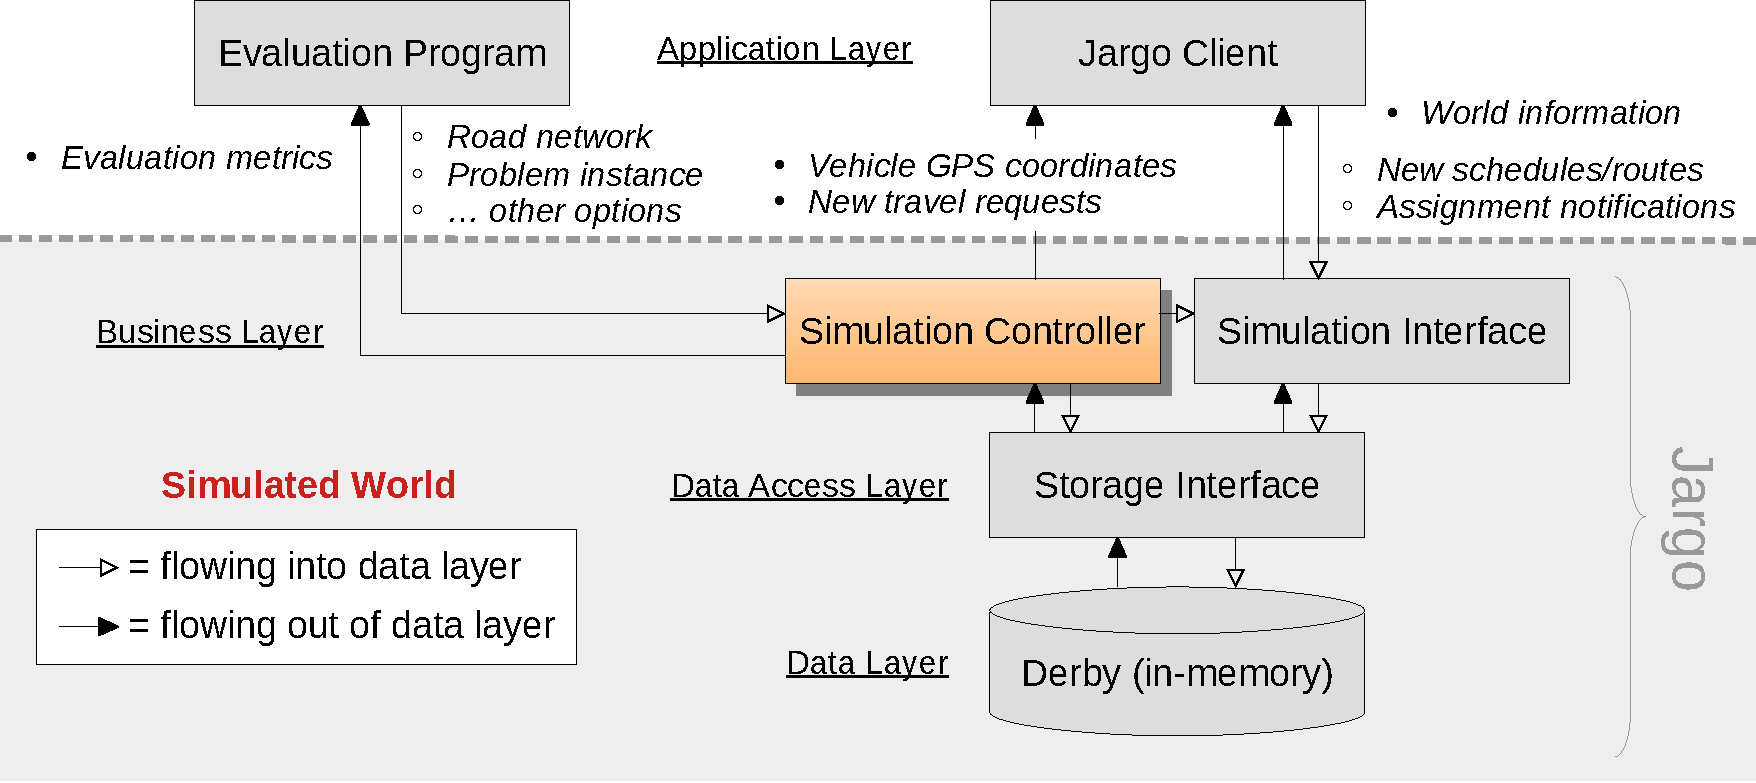
\includegraphics[width=150mm]{src/fig/controller-fig}
\caption{Controller within the Jargo stack.}
\label{fig:controller}
\end{figure}

\section{Implementation Overview}
The code consist of the \emph{preamble} (\S\ref{sec:preamble})
and the \emph{class definition} (\S\ref{sec:class-definition}).
\nwfilename{src/Controller.nw}\nwbegincode{1}\sublabel{NW2ZDXo8-34QoYM-1}\nwmargintag{{\nwtagstyle{}\subpageref{NW2ZDXo8-34QoYM-1}}}\moddef{Controller.java~{\nwtagstyle{}\subpageref{NW2ZDXo8-34QoYM-1}}}\endmoddef\nwnotused{Controller.java}
\LA{}Controller.java preamble~{\nwtagstyle{}\subpageref{NW2ZDXo8-m6OHq-1}}\RA{}
\LA{}\code{}Controller\edoc{} definition~{\nwtagstyle{}\subpageref{NW2ZDXo8-3kvp2C-1}}\RA{}
\nwendcode{}\nwbegindocs{2}\nwdocspar

\subsection{Preamble}
\label{sec:preamble}
The preamble declares the package and imports dependencies.
\nwenddocs{}\nwbegincode{3}\sublabel{NW2ZDXo8-m6OHq-1}\nwmargintag{{\nwtagstyle{}\subpageref{NW2ZDXo8-m6OHq-1}}}\moddef{Controller.java preamble~{\nwtagstyle{}\subpageref{NW2ZDXo8-m6OHq-1}}}\endmoddef\nwalsodefined{\\{NW2ZDXo8-m6OHq-2}\\{NW2ZDXo8-m6OHq-3}\\{NW2ZDXo8-m6OHq-4}\\{NW2ZDXo8-m6OHq-5}\\{NW2ZDXo8-m6OHq-6}}\nwused{\\{NW2ZDXo8-34QoYM-1}}
package com.github.jargors;
\nwendcode{}\nwbegindocs{4}\nwdocspar
We import:
\begin{itemize}
\item all parts of the Jargo stack;
\nwenddocs{}\nwbegincode{5}\sublabel{NW2ZDXo8-m6OHq-2}\nwmargintag{{\nwtagstyle{}\subpageref{NW2ZDXo8-m6OHq-2}}}\moddef{Controller.java preamble~{\nwtagstyle{}\subpageref{NW2ZDXo8-m6OHq-1}}}\plusendmoddef
import com.github.jargors.Storage;
import com.github.jargors.Communicator;
import com.github.jargors.Client;
import com.github.jargors.Tools;
import com.github.jargors.exceptions.ClientException;
import com.github.jargors.exceptions.ClientFatalException;
import com.github.jargors.exceptions.DuplicateVertexException;
import com.github.jargors.exceptions.DuplicateEdgeException;
import com.github.jargors.exceptions.DuplicateUserException;
import com.github.jargors.exceptions.EdgeNotFoundException;
import com.github.jargors.exceptions.UserNotFoundException;
import com.github.jargors.exceptions.VertexNotFoundException;
\nwendcode{}\nwbegindocs{6}\item standard utilities for concurrent execution;
\nwenddocs{}\nwbegincode{7}\sublabel{NW2ZDXo8-m6OHq-3}\nwmargintag{{\nwtagstyle{}\subpageref{NW2ZDXo8-m6OHq-3}}}\moddef{Controller.java preamble~{\nwtagstyle{}\subpageref{NW2ZDXo8-m6OHq-1}}}\plusendmoddef
import java.util.concurrent.CompletableFuture;
import java.util.concurrent.Executors;
import java.util.concurrent.ScheduledExecutorService;
import java.util.concurrent.ScheduledFuture;
import java.util.concurrent.TimeUnit;
import java.util.function.Consumer;
\nwendcode{}\nwbegindocs{8}\item standard classes for file operations;
\nwenddocs{}\nwbegincode{9}\sublabel{NW2ZDXo8-m6OHq-4}\nwmargintag{{\nwtagstyle{}\subpageref{NW2ZDXo8-m6OHq-4}}}\moddef{Controller.java preamble~{\nwtagstyle{}\subpageref{NW2ZDXo8-m6OHq-1}}}\plusendmoddef
import java.util.Scanner;
import java.io.File;
import java.io.FileNotFoundException;
\nwendcode{}\nwbegindocs{10}\item standard map classes for caching various items.
\nwenddocs{}\nwbegincode{11}\sublabel{NW2ZDXo8-m6OHq-5}\nwmargintag{{\nwtagstyle{}\subpageref{NW2ZDXo8-m6OHq-5}}}\moddef{Controller.java preamble~{\nwtagstyle{}\subpageref{NW2ZDXo8-m6OHq-1}}}\plusendmoddef
import java.util.Map;
import java.util.HashMap;
\nwendcode{}\nwbegindocs{12}\nwdocspar
\nwenddocs{}\nwbegincode{13}\sublabel{NW2ZDXo8-m6OHq-6}\nwmargintag{{\nwtagstyle{}\subpageref{NW2ZDXo8-m6OHq-6}}}\moddef{Controller.java preamble~{\nwtagstyle{}\subpageref{NW2ZDXo8-m6OHq-1}}}\plusendmoddef
import java.sql.SQLException;
\nwendcode{}\nwbegindocs{14}\nwdocspar
\end{itemize}

\subsection{Class Definition}
\label{sec:class-definition}
\nwenddocs{}\nwbegincode{15}\sublabel{NW2ZDXo8-3kvp2C-1}\nwmargintag{{\nwtagstyle{}\subpageref{NW2ZDXo8-3kvp2C-1}}}\moddef{\code{}Controller\edoc{} definition~{\nwtagstyle{}\subpageref{NW2ZDXo8-3kvp2C-1}}}\endmoddef\nwused{\\{NW2ZDXo8-34QoYM-1}}
public class Controller \{
  \LA{}\code{}Controller\edoc{} member variables~{\nwtagstyle{}\subpageref{NW2ZDXo8-3yXfwG-1}}\RA{}
  \LA{}\code{}Controller\edoc{} constructor~{\nwtagstyle{}\subpageref{NW2ZDXo8-3AyyZG-1}}\RA{}
  \LA{}\code{}Controller\edoc{} public methods~{\nwtagstyle{}\subpageref{NW2ZDXo8-bF3Hn-1}}\RA{}
\}
\nwendcode{}\nwbegindocs{16}\nwdocspar

\subsection{Member Variables}
Member variables are grouped into \emph{containers}, \emph{settings}, and
\emph{loops}.
\nwenddocs{}\nwbegincode{17}\sublabel{NW2ZDXo8-3yXfwG-1}\nwmargintag{{\nwtagstyle{}\subpageref{NW2ZDXo8-3yXfwG-1}}}\moddef{\code{}Controller\edoc{} member variables~{\nwtagstyle{}\subpageref{NW2ZDXo8-3yXfwG-1}}}\endmoddef\nwused{\\{NW2ZDXo8-3kvp2C-1}}
\LA{}Container objects~{\nwtagstyle{}\subpageref{NW2ZDXo8-OUspt-1}}\RA{}
\LA{}Settings objects~{\nwtagstyle{}\subpageref{NW2ZDXo8-2svhLD-1}}\RA{}
\LA{}Loop objects~{\nwtagstyle{}\subpageref{NW2ZDXo8-2e0Sfa-1}}\RA{}
\nwendcode{}\nwbegindocs{18}\nwdocspar
\hi{Containers.}
\nwenddocs{}\nwbegincode{19}\sublabel{NW2ZDXo8-OUspt-1}\nwmargintag{{\nwtagstyle{}\subpageref{NW2ZDXo8-OUspt-1}}}\moddef{Container objects~{\nwtagstyle{}\subpageref{NW2ZDXo8-OUspt-1}}}\endmoddef\nwused{\\{NW2ZDXo8-3yXfwG-1}}
private Storage storage;
private Communicator communicator;
private Tools tools = new Tools();
private Client client;
private Map<Integer, Boolean> lu_seen = new HashMap<>();
\nwindexdefn{storage}{storage}{NW2ZDXo8-OUspt-1}\nwindexdefn{communicator}{communicator}{NW2ZDXo8-OUspt-1}\nwindexdefn{tools}{tools}{NW2ZDXo8-OUspt-1}\nwindexdefn{client}{client}{NW2ZDXo8-OUspt-1}\nwindexdefn{lu{\char95}seen}{lu:unseen}{NW2ZDXo8-OUspt-1}\eatline
\nwidentdefs{\\{{client}{client}}\\{{communicator}{communicator}}\\{{lu{\char95}seen}{lu:unseen}}\\{{storage}{storage}}\\{{tools}{tools}}}\nwendcode{}\nwbegindocs{20}\nwdocspar
\hi{Settings.} Settings objects configure various aspects of the simulation.
Some settings can be configured using the public setters, others can
be configured through system properties, and others are non-configurable.
\nwenddocs{}\nwbegincode{21}\sublabel{NW2ZDXo8-2svhLD-1}\nwmargintag{{\nwtagstyle{}\subpageref{NW2ZDXo8-2svhLD-1}}}\moddef{Settings objects~{\nwtagstyle{}\subpageref{NW2ZDXo8-2svhLD-1}}}\endmoddef\nwalsodefined{\\{NW2ZDXo8-2svhLD-2}\\{NW2ZDXo8-2svhLD-3}\\{NW2ZDXo8-2svhLD-4}\\{NW2ZDXo8-2svhLD-5}}\nwused{\\{NW2ZDXo8-3yXfwG-1}}
private int initial_world_time = 0;
private int final_world_time = 86400;
\nwindexdefn{initial{\char95}world{\char95}time}{initial:unworld:untime}{NW2ZDXo8-2svhLD-1}\nwindexdefn{final{\char95}world{\char95}time}{final:unworld:untime}{NW2ZDXo8-2svhLD-1}\eatline
\nwidentdefs{\\{{final{\char95}world{\char95}time}{final:unworld:untime}}\\{{initial{\char95}world{\char95}time}{initial:unworld:untime}}}\nwendcode{}\nwbegindocs{22}The simulation world time is stored in {\tt{}\protect\nwindexuse{world{\char95}time}{world:untime}{NW2ZDXo8-2svhLD-2}world{\char95}time} and is upated by the
clock loop. The time advances in increments of 1 from {\tt{}\protect\nwindexuse{initial{\char95}world{\char95}time}{initial:unworld:untime}{NW2ZDXo8-2svhLD-1}initial{\char95}world{\char95}time}
to {\tt{}\protect\nwindexuse{final{\char95}world{\char95}time}{final:unworld:untime}{NW2ZDXo8-2svhLD-1}final{\char95}world{\char95}time}.
\nwenddocs{}\nwbegincode{23}\sublabel{NW2ZDXo8-2svhLD-2}\nwmargintag{{\nwtagstyle{}\subpageref{NW2ZDXo8-2svhLD-2}}}\moddef{Settings objects~{\nwtagstyle{}\subpageref{NW2ZDXo8-2svhLD-1}}}\plusendmoddef
private int world_time = 0;
\nwindexdefn{world{\char95}time}{world:untime}{NW2ZDXo8-2svhLD-2}\eatline
\nwidentdefs{\\{{world{\char95}time}{world:untime}}}\nwendcode{}\nwbegindocs{24}The {\tt{}\protect\nwindexuse{loop{\char95}delay}{loop:undelay}{NW2ZDXo8-2svhLD-3}loop{\char95}delay} configures how many seconds to wait until the controller
loops start. The update periods configure how often particular loops should
execute, in seconds.
\nwenddocs{}\nwbegincode{25}\sublabel{NW2ZDXo8-2svhLD-3}\nwmargintag{{\nwtagstyle{}\subpageref{NW2ZDXo8-2svhLD-3}}}\moddef{Settings objects~{\nwtagstyle{}\subpageref{NW2ZDXo8-2svhLD-1}}}\plusendmoddef
private int loop_delay = 0;
private int engine_update_period = 10;
// private int deviation_rate = 0.02;
// private int breakdown_rate = 0.005;
\nwindexdefn{loop{\char95}delay}{loop:undelay}{NW2ZDXo8-2svhLD-3}\nwindexdefn{engine{\char95}update{\char95}period}{engine:unupdate:unperiod}{NW2ZDXo8-2svhLD-3}\eatline
\nwidentdefs{\\{{engine{\char95}update{\char95}period}{engine:unupdate:unperiod}}\\{{loop{\char95}delay}{loop:undelay}}}\nwendcode{}\nwbegindocs{26}The {\tt{}\protect\nwindexuse{CSHIFT}{CSHIFT}{NW2ZDXo8-2svhLD-4}CSHIFT} setting configures the precision for longitude and latitude
coordiates (see {\tt{}Storage.DBAddNewVertex}(3))\footnote{Beware, if {\tt{}\protect\nwindexuse{CSHIFT}{CSHIFT}{NW2ZDXo8-2svhLD-4}CSHIFT}
is changed here, it should also be changed in Tools.}.
\nwenddocs{}\nwbegincode{27}\sublabel{NW2ZDXo8-2svhLD-4}\nwmargintag{{\nwtagstyle{}\subpageref{NW2ZDXo8-2svhLD-4}}}\moddef{Settings objects~{\nwtagstyle{}\subpageref{NW2ZDXo8-2svhLD-1}}}\plusendmoddef
private final double CSHIFT = 10000000.0;
\nwindexdefn{CSHIFT}{CSHIFT}{NW2ZDXo8-2svhLD-4}\eatline
\nwidentdefs{\\{{CSHIFT}{CSHIFT}}}\nwendcode{}\nwbegindocs{28}The {\tt{}\protect\nwindexuse{DEBUG}{DEBUG}{NW2ZDXo8-2svhLD-5}DEBUG} setting controls whether certain messages are print to screen.
Pass {\tt{}-Djargors.controller.debug=true} to the {\tt{}java} command to set
{\tt{}\protect\nwindexuse{DEBUG}{DEBUG}{NW2ZDXo8-2svhLD-5}DEBUG} to {\tt{}true}.
\nwenddocs{}\nwbegincode{29}\sublabel{NW2ZDXo8-2svhLD-5}\nwmargintag{{\nwtagstyle{}\subpageref{NW2ZDXo8-2svhLD-5}}}\moddef{Settings objects~{\nwtagstyle{}\subpageref{NW2ZDXo8-2svhLD-1}}}\plusendmoddef
private final boolean DEBUG = "true".equals(System.getProperty("jargors.controller.debug"));
\nwindexdefn{DEBUG}{DEBUG}{NW2ZDXo8-2svhLD-5}\eatline
\nwidentdefs{\\{{DEBUG}{DEBUG}}}\nwendcode{}\nwbegindocs{30}\nwdocspar
\hi{Loops.} Jargo's simulation environment comprises four ``loops'', defined
here, running in parallel. They are executed using Java's
{\tt{}ScheduledExecutorService} to control timing.
\nwenddocs{}\nwbegincode{31}\sublabel{NW2ZDXo8-2e0Sfa-1}\nwmargintag{{\nwtagstyle{}\subpageref{NW2ZDXo8-2e0Sfa-1}}}\moddef{Loop objects~{\nwtagstyle{}\subpageref{NW2ZDXo8-2e0Sfa-1}}}\endmoddef\nwused{\\{NW2ZDXo8-3yXfwG-1}}
\LA{}Definition of clock loop~{\nwtagstyle{}\subpageref{NW2ZDXo8-2lFPcZ-1}}\RA{}
\LA{}Definition of engine loop~{\nwtagstyle{}\subpageref{NW2ZDXo8-3rcRXt-1}}\RA{}
\LA{}Definition of request collection loop~{\nwtagstyle{}\subpageref{NW2ZDXo8-10L3rI-1}}\RA{}
\LA{}Definition of request handling loop~{\nwtagstyle{}\subpageref{NW2ZDXo8-183plv-1}}\RA{}
\LA{}Definition of server collection loop~{\nwtagstyle{}\subpageref{NW2ZDXo8-1I3SnY-1}}\RA{}
\nwendcode{}\nwbegindocs{32}\nwdocspar

\subsubsection{Clock Loop}
\begin{tabular}{p{\textwidth}}
\toprule
\rowcolor{TableTitle}
Member \textcolor{blue}{{\tt{}\protect\nosublabel{NW2ZDXo8-2e0Sfa-1-u5}\protect\nwindexuse{ClockLoop}{ClockLoop}{NW2ZDXo8-2lFPcZ-1}ClockLoop}} is a {\tt{}Runnable} that does two things.
First it advances the simulation world time, and then it tells {\tt{}\protect\nwindexuse{communicator}{communicator}{NW2ZDXo8-OUspt-1}communicator}
about the new time.\\
\midrule
\textbf{Parameters:} none.\\
\textbf{Returns:} nothing.\\
\textbf{Side Effects:} increments {\tt{}\protect\nwindexuse{world{\char95}time}{world:untime}{NW2ZDXo8-2svhLD-2}world{\char95}time} by 1, may modify
{\tt{}\protect\nwindexuse{communicator}{communicator}{NW2ZDXo8-OUspt-1}communicator} by changing {\tt{}Communicator.\protect\nwindexuse{world{\char95}time}{world:untime}{NW2ZDXo8-2svhLD-2}world{\char95}time}, may print to
standard error if {\tt{}\protect\nwindexuse{DEBUG}{DEBUG}{NW2ZDXo8-2svhLD-5}DEBUG} is {\tt{}true}.\\
\textbf{Throws:} nothing.\\
\bottomrule
\end{tabular}
\nwenddocs{}\nwbegincode{33}\sublabel{NW2ZDXo8-2lFPcZ-1}\nwmargintag{{\nwtagstyle{}\subpageref{NW2ZDXo8-2lFPcZ-1}}}\moddef{Definition of clock loop~{\nwtagstyle{}\subpageref{NW2ZDXo8-2lFPcZ-1}}}\endmoddef\nwused{\\{NW2ZDXo8-2e0Sfa-1}}
private Runnable ClockLoop = () -> \{
  this.communicator.setSimulationWorldTime(++(this.world_time));
  if (DEBUG) \{
    System.err.printf("[t=%d] Controller.ClockLoop says: %s!",
        this.world_time, (this.world_time % 2 == 0 ? "ping" : "pong"));
  \}
\};
\nwindexdefn{ClockLoop}{ClockLoop}{NW2ZDXo8-2lFPcZ-1}\eatline
\nwidentdefs{\\{{ClockLoop}{ClockLoop}}}\nwidentuses{\\{{communicator}{communicator}}\\{{DEBUG}{DEBUG}}\\{{world{\char95}time}{world:untime}}}\nwindexuse{communicator}{communicator}{NW2ZDXo8-2lFPcZ-1}\nwindexuse{DEBUG}{DEBUG}{NW2ZDXo8-2lFPcZ-1}\nwindexuse{world{\char95}time}{world:untime}{NW2ZDXo8-2lFPcZ-1}\nwendcode{}\nwbegindocs{34}\nwdocspar
\subsubsection{Engine Loop}
\begin{tabular}{p{\textwidth}}
\toprule
\rowcolor{TableTitle}
Member \textcolor{blue}{{\tt{}\protect\nwindexuse{EngineLoop}{EngineLoop}{NW2ZDXo8-3rcRXt-1}EngineLoop}} is a {\tt{}Runnable} that simulates
stochastic effects on the ridesharing vehicles.\\
\midrule
\textbf{Parameters:} none.\\
\textbf{Returns:} nothing.\\
\textbf{Side Effects:} may insert, delete, or update rows in Tables W, CW,
PD, CPD, and CQ in the database instance underlying {\tt{}\protect\nwindexuse{storage}{storage}{NW2ZDXo8-OUspt-1}storage}.\\
\textbf{Throws:} nothing.\\
\bottomrule
\end{tabular}
\nwenddocs{}\nwbegincode{35}\sublabel{NW2ZDXo8-3rcRXt-1}\nwmargintag{{\nwtagstyle{}\subpageref{NW2ZDXo8-3rcRXt-1}}}\moddef{Definition of engine loop~{\nwtagstyle{}\subpageref{NW2ZDXo8-3rcRXt-1}}}\endmoddef\nwused{\\{NW2ZDXo8-2e0Sfa-1}}
private Runnable EngineLoop = () -> \{
  // Idea: what if we apply traffic effects at the time a server route is
  // submitted? we can do it because we know what the future traffic will
  // be and we also know where the future location will be of the server.
  // then, is this loop necessary?
\};
\nwindexdefn{EngineLoop}{EngineLoop}{NW2ZDXo8-3rcRXt-1}\eatline
\nwidentdefs{\\{{EngineLoop}{EngineLoop}}}\nwendcode{}\nwbegindocs{36}\nwdocspar
\subsubsection{Request Collection Loop}
\begin{tabular}{p{\textwidth}}
\toprule
\rowcolor{TableTitle}
Member \textcolor{blue}{{\tt{}\protect\nwindexuse{RequestCollectionLoop}{RequestCollectionLoop}{NW2ZDXo8-10L3rI-1}RequestCollectionLoop}} is a {\tt{}Runnable} that
collects requests eligible for assignment at the current world time.  A request
$r$ is ``eligible'' if it is not assigned at the current world time, and if the
world time is between the request's early time $r_\texttt{e}$ and
$(r_\texttt{e}+\texttt{REQUEST\_TIMEOUT})$ (see
{\tt{}Storage.DBQueryQueuedRequests}(1)). If the eligible requests cannot be
collected, we consider this failure to be fatal and exit immediately. A possible
reason may be database failure in {\tt{}\protect\nwindexuse{storage}{storage}{NW2ZDXo8-OUspt-1}storage}. \\
\midrule
\textbf{Parameters:} none.\\
\textbf{Returns:} nothing.\\
\textbf{Side Effects:} may modify {\tt{}\protect\nwindexuse{client}{client}{NW2ZDXo8-OUspt-1}client} by adding objects into
{\tt{}Client.queue}, may put new entries or modify existing entries in
{\tt{}\protect\nwindexuse{lu{\char95}seen}{lu:unseen}{NW2ZDXo8-OUspt-1}lu{\char95}seen}, may print to standard error if {\tt{}\protect\nwindexuse{DEBUG}{DEBUG}{NW2ZDXo8-2svhLD-5}DEBUG} is {\tt{}true}, or exits the JVM if
failure occurs.\\
\textbf{Throws:} nothing.\\
\bottomrule
\end{tabular}
\nwenddocs{}\nwbegincode{37}\sublabel{NW2ZDXo8-10L3rI-1}\nwmargintag{{\nwtagstyle{}\subpageref{NW2ZDXo8-10L3rI-1}}}\moddef{Definition of request collection loop~{\nwtagstyle{}\subpageref{NW2ZDXo8-10L3rI-1}}}\endmoddef\nwused{\\{NW2ZDXo8-2e0Sfa-1}}
private Runnable RequestCollectionLoop = () -> \{
  long A0 = 0;
  if (DEBUG) \{
    A0 = System.currentTimeMillis();
  \}
  try \{
    int[] output = this.storage.DBQueryQueuedRequests(this.world_time);
    for (int i = 0; i < (output.length - 6); i += 7) \{
      if (!this.lu_seen.containsKey(output[i]) || this.lu_seen.get(output[i]) == false) \{
        this.client.collectRequest(new int[] \{
          output[(i + 0)],
          output[(i + 1)],
          output[(i + 2)],
          output[(i + 3)],
          output[(i + 4)],
          output[(i + 5)],
          output[(i + 6)] \});
        this.lu_seen.put(output[i], true);
      \}
    \}
  \} catch (SQLException e) \{
    System.err.println("Encountered fatal error");
    System.err.println(e.toString());
    e.printStackTrace();
    System.exit(1);
  \}
  if (DEBUG) \{
    System.err.printf("Controller.RequestCollectionLoop completed in %d ms\\n",
        (System.currentTimeMillis() - A0));
  \}
\};
\nwindexdefn{RequestCollectionLoop}{RequestCollectionLoop}{NW2ZDXo8-10L3rI-1}\eatline
\nwidentdefs{\\{{RequestCollectionLoop}{RequestCollectionLoop}}}\nwidentuses{\\{{client}{client}}\\{{DEBUG}{DEBUG}}\\{{lu{\char95}seen}{lu:unseen}}\\{{storage}{storage}}\\{{world{\char95}time}{world:untime}}}\nwindexuse{client}{client}{NW2ZDXo8-10L3rI-1}\nwindexuse{DEBUG}{DEBUG}{NW2ZDXo8-10L3rI-1}\nwindexuse{lu{\char95}seen}{lu:unseen}{NW2ZDXo8-10L3rI-1}\nwindexuse{storage}{storage}{NW2ZDXo8-10L3rI-1}\nwindexuse{world{\char95}time}{world:untime}{NW2ZDXo8-10L3rI-1}\nwendcode{}\nwbegindocs{38}\nwdocspar
\subsubsection{Request Handling Loop}
\begin{tabular}{p{\textwidth}}
\toprule
\rowcolor{TableTitle}
Member \textcolor{blue}{{\tt{}\protect\nwindexuse{RequestHandlingLoop}{RequestHandlingLoop}{NW2ZDXo8-183plv-1}RequestHandlingLoop}} is a {\tt{}Runnable} that
notifies the client algorithm to check for and process new requests.\\
\midrule
\textbf{Parameters:} none.\\
\textbf{Returns:} nothing.\\
\textbf{Side Effects:} may indirectly modify the database underlying
{\tt{}\protect\nwindexuse{storage}{storage}{NW2ZDXo8-OUspt-1}storage} depending on the body of {\tt{}Client.notifyNew}(0). May print to
standard error if a {\tt{}ClientException} occurs or {\tt{}ClientFatalException}
occurs or {\tt{}\protect\nwindexuse{DEBUG}{DEBUG}{NW2ZDXo8-2svhLD-5}DEBUG} is {\tt{}true}, or exits the JVM if {\tt{}ClientFatalException}
occurs.\\
\textbf{Throws:} nothing.\\
\bottomrule
\end{tabular}
\nwenddocs{}\nwbegincode{39}\sublabel{NW2ZDXo8-183plv-1}\nwmargintag{{\nwtagstyle{}\subpageref{NW2ZDXo8-183plv-1}}}\moddef{Definition of request handling loop~{\nwtagstyle{}\subpageref{NW2ZDXo8-183plv-1}}}\endmoddef\nwused{\\{NW2ZDXo8-2e0Sfa-1}}
private Runnable RequestHandlingLoop = () -> \{
  long A0 = 0;
  if (DEBUG) \{
    A0 = System.currentTimeMillis();
  \}
  try \{
    this.client.notifyNew();
  \} catch (ClientException e) \{
    System.err.printf("[t=%d] Controller.RequestHandlingLoop caught a non-fatal Client exception: %s",
        this.world_time, e.toString());
  \} catch (ClientFatalException e) \{
    System.err.printf("[t=%d] Controller.RequestHandlingLoop caught a FATAL Client exception: %s",
        this.world_time, e.toString());
    e.printStackTrace();
    System.exit(1);
  \}
  if (DEBUG) \{
    System.err.printf("Controller.RequestHandlingLoop completed in %d ms\\n",
        (System.currentTimeMillis() - A0));
  \}
\};
\nwindexdefn{RequestHandlingLoop}{RequestHandlingLoop}{NW2ZDXo8-183plv-1}\eatline
\nwidentdefs{\\{{RequestHandlingLoop}{RequestHandlingLoop}}}\nwidentuses{\\{{client}{client}}\\{{DEBUG}{DEBUG}}\\{{world{\char95}time}{world:untime}}}\nwindexuse{client}{client}{NW2ZDXo8-183plv-1}\nwindexuse{DEBUG}{DEBUG}{NW2ZDXo8-183plv-1}\nwindexuse{world{\char95}time}{world:untime}{NW2ZDXo8-183plv-1}\nwendcode{}\nwbegindocs{40}\nwdocspar
\subsubsection{Server Loop}
\begin{tabular}{p{\textwidth}}
\toprule
\rowcolor{TableTitle}
Member \textcolor{blue}{{\tt{}\protect\nwindexuse{ServerLoop}{ServerLoop}{NW2ZDXo8-1I3SnY-1}ServerLoop}} is a {\tt{}Runnable} that collects
last-known locations of all active servers at the current word time.  A server
is ``active'' if its service has not ended, in other words it has not arrived
at its own destination.  The ``last-known location'' is the waypoint in the
server's route $w$ with a time component closest to but not exceeding the given
time, in other words ${w_{\leq t}}_{|w_{\leq t}|}$ (see
{\tt{}Storage.DBQueryServerLocationsActive}(1)).  If the last-known locations
cannot be collected, we consider this failure to be fatal and exit immediately.
A possible reason may be database failure in {\tt{}\protect\nwindexuse{storage}{storage}{NW2ZDXo8-OUspt-1}storage}. \\
\midrule
\textbf{Parameters:} none.\\
\textbf{Returns:} nothing.\\
\textbf{Side Effects:} may indirectly modify the database underlying
{\tt{}\protect\nwindexuse{storage}{storage}{NW2ZDXo8-OUspt-1}storage} depending on the body of {\tt{}Client.collectServerLocations}(1).
May print to standard error if {\tt{}\protect\nwindexuse{DEBUG}{DEBUG}{NW2ZDXo8-2svhLD-5}DEBUG} is {\tt{}true}, or
exits the JVM if failure occurs.\\
\textbf{Throws:} nothing.\\
\bottomrule
\end{tabular}
\nwenddocs{}\nwbegincode{41}\sublabel{NW2ZDXo8-1I3SnY-1}\nwmargintag{{\nwtagstyle{}\subpageref{NW2ZDXo8-1I3SnY-1}}}\moddef{Definition of server collection loop~{\nwtagstyle{}\subpageref{NW2ZDXo8-1I3SnY-1}}}\endmoddef\nwused{\\{NW2ZDXo8-2e0Sfa-1}}
private Runnable ServerLoop = () -> \{
  long A0 = 0;
  if (DEBUG) \{
    A0 = System.currentTimeMillis();
  \}
  try \{
    int[] output = this.storage.DBQueryServerLocationsActive(this.world_time);
    this.client.collectServerLocations(output);
  \} catch (SQLException e) \{
    System.err.println("Encountered fatal error");
    System.err.println(e.toString());
    e.printStackTrace();
    System.exit(1);
  \}
  if (DEBUG) \{
    System.err.printf("Controller.ServerLoop completed in %d ms\\n",
        (System.currentTimeMillis() - A0));
  \}
\};
\nwindexdefn{ServerLoop}{ServerLoop}{NW2ZDXo8-1I3SnY-1}\eatline
\nwidentdefs{\\{{ServerLoop}{ServerLoop}}}\nwidentuses{\\{{client}{client}}\\{{DEBUG}{DEBUG}}\\{{storage}{storage}}\\{{world{\char95}time}{world:untime}}}\nwindexuse{client}{client}{NW2ZDXo8-1I3SnY-1}\nwindexuse{DEBUG}{DEBUG}{NW2ZDXo8-1I3SnY-1}\nwindexuse{storage}{storage}{NW2ZDXo8-1I3SnY-1}\nwindexuse{world{\char95}time}{world:untime}{NW2ZDXo8-1I3SnY-1}\nwendcode{}\nwbegindocs{42}\nwdocspar
\subsection{Constructor}
\begin{tabular}{p{\textwidth}}
\toprule
\rowcolor{TableTitle}
Constructor \textcolor{blue}{{\tt{}Controller}}(0) registers a new {\tt{}Storage} to
the {\tt{}\protect\nwindexuse{storage}{storage}{NW2ZDXo8-OUspt-1}storage} member variable. It also registers a new {\tt{}Communicator} to
the {\tt{}\protect\nwindexuse{communicator}{communicator}{NW2ZDXo8-OUspt-1}communicator} member variable. It then registers itself and the new
{\tt{}Storage} to {\tt{}\protect\nwindexuse{communicator}{communicator}{NW2ZDXo8-OUspt-1}communicator}.\\
\midrule
\textbf{Parameters:} none.\\
\textbf{Returns:} nothing.\\
\textbf{Side Effects:} creates a new {\tt{}Storage} and {\tt{}Communicator} on the
memory heap, modifies {\tt{}\protect\nwindexuse{storage}{storage}{NW2ZDXo8-OUspt-1}storage} and {\tt{}\protect\nwindexuse{communicator}{communicator}{NW2ZDXo8-OUspt-1}communicator}.\\
\textbf{Throws:} nothing.\\
\bottomrule
\end{tabular}
\nwenddocs{}\nwbegincode{43}\sublabel{NW2ZDXo8-3AyyZG-1}\nwmargintag{{\nwtagstyle{}\subpageref{NW2ZDXo8-3AyyZG-1}}}\moddef{\code{}Controller\edoc{} constructor~{\nwtagstyle{}\subpageref{NW2ZDXo8-3AyyZG-1}}}\endmoddef\nwused{\\{NW2ZDXo8-3kvp2C-1}}
public Controller() \{
  this.storage = new Storage();
  this.communicator = new Communicator();
  this.communicator.registerStorage(storage);
  this.communicator.registerController(this);
\}
\nwidentuses{\\{{communicator}{communicator}}\\{{storage}{storage}}}\nwindexuse{communicator}{communicator}{NW2ZDXo8-3AyyZG-1}\nwindexuse{storage}{storage}{NW2ZDXo8-3AyyZG-1}\nwendcode{}\nwbegindocs{44}\nwdocspar

\section{Public Methods}
\label{sec:public-methods}
\hi{General methods.}
\nwenddocs{}\nwbegincode{45}\sublabel{NW2ZDXo8-bF3Hn-1}\nwmargintag{{\nwtagstyle{}\subpageref{NW2ZDXo8-bF3Hn-1}}}\moddef{\code{}Controller\edoc{} public methods~{\nwtagstyle{}\subpageref{NW2ZDXo8-bF3Hn-1}}}\endmoddef\nwalsodefined{\\{NW2ZDXo8-bF3Hn-2}\\{NW2ZDXo8-bF3Hn-3}}\nwused{\\{NW2ZDXo8-3kvp2C-1}}
\LA{}Initialize new empty database~{\nwtagstyle{}\subpageref{NW2ZDXo8-2CVxut-1}}\RA{}
\LA{}Close database~{\nwtagstyle{}\subpageref{NW2ZDXo8-3A3oOU-1}}\RA{}
\LA{}Set client~{\nwtagstyle{}\subpageref{NW2ZDXo8-3HnCZ3-1}}\RA{}
\LA{}Set initial world time~{\nwtagstyle{}\subpageref{NW2ZDXo8-3BZAWj-1}}\RA{}
\LA{}Set final world time~{\nwtagstyle{}\subpageref{NW2ZDXo8-2PAB4K-1}}\RA{}
\LA{}Set engine update period~{\nwtagstyle{}\subpageref{NW2ZDXo8-2gxuga-1}}\RA{}
\LA{}Get world time~{\nwtagstyle{}\subpageref{NW2ZDXo8-3X8zhz-1}}\RA{}
\LA{}Return request to queue~{\nwtagstyle{}\subpageref{NW2ZDXo8-3SURrj-1}}\RA{}
\LA{}Save backup~{\nwtagstyle{}\subpageref{NW2ZDXo8-2OKmqF-1}}\RA{}
\LA{}Load backup~{\nwtagstyle{}\subpageref{NW2ZDXo8-b3Hn1-1}}\RA{}
\LA{}Load data model~{\nwtagstyle{}\subpageref{NW2ZDXo8-4P4YpK-1}}\RA{}
\LA{}Load road network~{\nwtagstyle{}\subpageref{NW2ZDXo8-1JUvcB-1}}\RA{}
\LA{}Load problem~{\nwtagstyle{}\subpageref{NW2ZDXo8-2rtVpi-1}}\RA{}
\LA{}Load GTree~{\nwtagstyle{}\subpageref{NW2ZDXo8-b7Jka-1}}\RA{}
\LA{}Start dynamic simulation~{\nwtagstyle{}\subpageref{NW2ZDXo8-43uvLJ-1}}\RA{}
\LA{}Start static simulation~{\nwtagstyle{}\subpageref{NW2ZDXo8-1n2dd-1}}\RA{}
\nwendcode{}\nwbegindocs{46}\nwdocspar
\hi{Read methods.}
\nwenddocs{}\nwbegincode{47}\sublabel{NW2ZDXo8-bF3Hn-2}\nwmargintag{{\nwtagstyle{}\subpageref{NW2ZDXo8-bF3Hn-2}}}\moddef{\code{}Controller\edoc{} public methods~{\nwtagstyle{}\subpageref{NW2ZDXo8-bF3Hn-1}}}\plusendmoddef
\LA{}Query custom statement~{\nwtagstyle{}\subpageref{NW2ZDXo8-2FtqIZ-1}}\RA{}
\LA{}Query all vertices~{\nwtagstyle{}\subpageref{NW2ZDXo8-1r5OnM-1}}\RA{}
\LA{}Query all edges~{\nwtagstyle{}\subpageref{NW2ZDXo8-4ILREc-1}}\RA{}
\LA{}Query vertex~{\nwtagstyle{}\subpageref{NW2ZDXo8-4IfXsG-1}}\RA{}
\LA{}Query edge~{\nwtagstyle{}\subpageref{NW2ZDXo8-1E2aru-1}}\RA{}
\LA{}Query ridesharing user~{\nwtagstyle{}\subpageref{NW2ZDXo8-3isdeu-1}}\RA{}
\LA{}Query queued requests~{\nwtagstyle{}\subpageref{NW2ZDXo8-3AGrxZ-1}}\RA{}
\LA{}Query routes~{\nwtagstyle{}\subpageref{NW2ZDXo8-1AprqI-1}}\RA{}
\LA{}Query schedules~{\nwtagstyle{}\subpageref{NW2ZDXo8-3yA8FQ-1}}\RA{}
\LA{}Query various metrics~{\nwtagstyle{}\subpageref{NW2ZDXo8-1Ang64-1}}\RA{}
\nwendcode{}\nwbegindocs{48}\nwdocspar
\hi{Write methods.}
\nwenddocs{}\nwbegincode{49}\sublabel{NW2ZDXo8-bF3Hn-3}\nwmargintag{{\nwtagstyle{}\subpageref{NW2ZDXo8-bF3Hn-3}}}\moddef{\code{}Controller\edoc{} public methods~{\nwtagstyle{}\subpageref{NW2ZDXo8-bF3Hn-1}}}\plusendmoddef
\LA{}Add new server~{\nwtagstyle{}\subpageref{NW2ZDXo8-IYVQQ-1}}\RA{}
\LA{}Add new request~{\nwtagstyle{}\subpageref{NW2ZDXo8-4ISWm4-1}}\RA{}
\nwendcode{}\nwbegindocs{50}\nwdocspar

\subsection{General methods}

\subsubsection{{\tt{}\protect\nosublabel{NW2ZDXo8-bF3Hn-3-u2}\protect\nwindexuse{createNewInstance}{createNewInstance}{NW2ZDXo8-2CVxut-1}createNewInstance}(0)}
\nwenddocs{}\nwbegincode{51}\sublabel{NW2ZDXo8-2CVxut-1}\nwmargintag{{\nwtagstyle{}\subpageref{NW2ZDXo8-2CVxut-1}}}\moddef{Initialize new empty database~{\nwtagstyle{}\subpageref{NW2ZDXo8-2CVxut-1}}}\endmoddef\nwused{\\{NW2ZDXo8-bF3Hn-1}}
public void createNewInstance() throws SQLException \{
  this.storage.DBCreateNewInstance();
\}
\nwindexdefn{createNewInstance}{createNewInstance}{NW2ZDXo8-2CVxut-1}\eatline
\nwidentdefs{\\{{createNewInstance}{createNewInstance}}}\nwidentuses{\\{{storage}{storage}}}\nwindexuse{storage}{storage}{NW2ZDXo8-2CVxut-1}\nwendcode{}\nwbegindocs{52}\nwdocspar
\subsubsection{{\tt{}\protect\nwindexuse{closeInstance}{closeInstance}{NW2ZDXo8-3A3oOU-1}closeInstance}(0)}
\nwenddocs{}\nwbegincode{53}\sublabel{NW2ZDXo8-3A3oOU-1}\nwmargintag{{\nwtagstyle{}\subpageref{NW2ZDXo8-3A3oOU-1}}}\moddef{Close database~{\nwtagstyle{}\subpageref{NW2ZDXo8-3A3oOU-1}}}\endmoddef\nwused{\\{NW2ZDXo8-bF3Hn-1}}
public void closeInstance() throws SQLException \{
  this.storage.DBCloseInstance();
\}
\nwindexdefn{closeInstance}{closeInstance}{NW2ZDXo8-3A3oOU-1}\eatline
\nwidentdefs{\\{{closeInstance}{closeInstance}}}\nwidentuses{\\{{storage}{storage}}}\nwindexuse{storage}{storage}{NW2ZDXo8-3A3oOU-1}\nwendcode{}\nwbegindocs{54}\nwdocspar
\subsubsection{{\tt{}\protect\nwindexuse{setClient}{setClient}{NW2ZDXo8-3HnCZ3-1}setClient}(1)}
\nwenddocs{}\nwbegincode{55}\sublabel{NW2ZDXo8-3HnCZ3-1}\nwmargintag{{\nwtagstyle{}\subpageref{NW2ZDXo8-3HnCZ3-1}}}\moddef{Set client~{\nwtagstyle{}\subpageref{NW2ZDXo8-3HnCZ3-1}}}\endmoddef\nwused{\\{NW2ZDXo8-bF3Hn-1}}
public void setClient(final Client target) \{
  this.client = target;
  this.client.setCommunicator(this.communicator);
\}
\nwindexdefn{setClient}{setClient}{NW2ZDXo8-3HnCZ3-1}\eatline
\nwidentdefs{\\{{setClient}{setClient}}}\nwidentuses{\\{{client}{client}}\\{{communicator}{communicator}}}\nwindexuse{client}{client}{NW2ZDXo8-3HnCZ3-1}\nwindexuse{communicator}{communicator}{NW2ZDXo8-3HnCZ3-1}\nwendcode{}\nwbegindocs{56}\nwdocspar
\subsubsection{{\tt{}\protect\nwindexuse{setInitialWorldTime}{setInitialWorldTime}{NW2ZDXo8-3BZAWj-1}setInitialWorldTime(1)}}
\nwenddocs{}\nwbegincode{57}\sublabel{NW2ZDXo8-3BZAWj-1}\nwmargintag{{\nwtagstyle{}\subpageref{NW2ZDXo8-3BZAWj-1}}}\moddef{Set initial world time~{\nwtagstyle{}\subpageref{NW2ZDXo8-3BZAWj-1}}}\endmoddef\nwused{\\{NW2ZDXo8-bF3Hn-1}}
public void setInitialWorldTime(final int t) \{
  this.initial_world_time = t;
\}
\nwindexdefn{setInitialWorldTime}{setInitialWorldTime}{NW2ZDXo8-3BZAWj-1}\eatline
\nwidentdefs{\\{{setInitialWorldTime}{setInitialWorldTime}}}\nwidentuses{\\{{initial{\char95}world{\char95}time}{initial:unworld:untime}}}\nwindexuse{initial{\char95}world{\char95}time}{initial:unworld:untime}{NW2ZDXo8-3BZAWj-1}\nwendcode{}\nwbegindocs{58}\nwdocspar
\subsubsection{{\tt{}\protect\nwindexuse{setFinalWorldTime}{setFinalWorldTime}{NW2ZDXo8-2PAB4K-1}setFinalWorldTime(1)}}
\nwenddocs{}\nwbegincode{59}\sublabel{NW2ZDXo8-2PAB4K-1}\nwmargintag{{\nwtagstyle{}\subpageref{NW2ZDXo8-2PAB4K-1}}}\moddef{Set final world time~{\nwtagstyle{}\subpageref{NW2ZDXo8-2PAB4K-1}}}\endmoddef\nwused{\\{NW2ZDXo8-bF3Hn-1}}
public void setFinalWorldTime(final int t) \{
  this.final_world_time = t;
\}
\nwindexdefn{setFinalWorldTime}{setFinalWorldTime}{NW2ZDXo8-2PAB4K-1}\eatline
\nwidentdefs{\\{{setFinalWorldTime}{setFinalWorldTime}}}\nwidentuses{\\{{final{\char95}world{\char95}time}{final:unworld:untime}}}\nwindexuse{final{\char95}world{\char95}time}{final:unworld:untime}{NW2ZDXo8-2PAB4K-1}\nwendcode{}\nwbegindocs{60}\nwdocspar
\subsubsection{{\tt{}\protect\nwindexuse{setEngineUpdatePeriod}{setEngineUpdatePeriod}{NW2ZDXo8-2gxuga-1}setEngineUpdatePeriod(1)}}
\nwenddocs{}\nwbegincode{61}\sublabel{NW2ZDXo8-2gxuga-1}\nwmargintag{{\nwtagstyle{}\subpageref{NW2ZDXo8-2gxuga-1}}}\moddef{Set engine update period~{\nwtagstyle{}\subpageref{NW2ZDXo8-2gxuga-1}}}\endmoddef\nwused{\\{NW2ZDXo8-bF3Hn-1}}
public void setEngineUpdatePeriod(final int t) \{
  this.engine_update_period = t;
\}
\nwindexdefn{setEngineUpdatePeriod}{setEngineUpdatePeriod}{NW2ZDXo8-2gxuga-1}\eatline
\nwidentdefs{\\{{setEngineUpdatePeriod}{setEngineUpdatePeriod}}}\nwidentuses{\\{{engine{\char95}update{\char95}period}{engine:unupdate:unperiod}}}\nwindexuse{engine{\char95}update{\char95}period}{engine:unupdate:unperiod}{NW2ZDXo8-2gxuga-1}\nwendcode{}\nwbegindocs{62}\nwdocspar
\subsubsection{{\tt{}\protect\nwindexuse{getSimulationWorldTime}{getSimulationWorldTime}{NW2ZDXo8-3X8zhz-1}getSimulationWorldTime(0)}}
\nwenddocs{}\nwbegincode{63}\sublabel{NW2ZDXo8-3X8zhz-1}\nwmargintag{{\nwtagstyle{}\subpageref{NW2ZDXo8-3X8zhz-1}}}\moddef{Get world time~{\nwtagstyle{}\subpageref{NW2ZDXo8-3X8zhz-1}}}\endmoddef\nwused{\\{NW2ZDXo8-bF3Hn-1}}
public int getSimulationWorldTime() \{
  return this.world_time;
\}
\nwindexdefn{getSimulationWorldTime}{getSimulationWorldTime}{NW2ZDXo8-3X8zhz-1}\eatline
\nwidentdefs{\\{{getSimulationWorldTime}{getSimulationWorldTime}}}\nwidentuses{\\{{world{\char95}time}{world:untime}}}\nwindexuse{world{\char95}time}{world:untime}{NW2ZDXo8-3X8zhz-1}\nwendcode{}\nwbegindocs{64}\nwdocspar

\subsubsection{{\tt{}\protect\nwindexuse{returnRequest}{returnRequest}{NW2ZDXo8-3SURrj-1}returnRequest}(1)}
\nwenddocs{}\nwbegincode{65}\sublabel{NW2ZDXo8-3SURrj-1}\nwmargintag{{\nwtagstyle{}\subpageref{NW2ZDXo8-3SURrj-1}}}\moddef{Return request to queue~{\nwtagstyle{}\subpageref{NW2ZDXo8-3SURrj-1}}}\endmoddef\nwused{\\{NW2ZDXo8-bF3Hn-1}}
public void returnRequest(final int rid) \{
  this.lu_seen.put(rid, false);
\}
\nwindexdefn{returnRequest}{returnRequest}{NW2ZDXo8-3SURrj-1}\eatline
\nwidentdefs{\\{{returnRequest}{returnRequest}}}\nwidentuses{\\{{lu{\char95}seen}{lu:unseen}}}\nwindexuse{lu{\char95}seen}{lu:unseen}{NW2ZDXo8-3SURrj-1}\nwendcode{}\nwbegindocs{66}\nwdocspar
\subsubsection{{\tt{}save}(1)}
\nwenddocs{}\nwbegincode{67}\sublabel{NW2ZDXo8-2OKmqF-1}\nwmargintag{{\nwtagstyle{}\subpageref{NW2ZDXo8-2OKmqF-1}}}\moddef{Save backup~{\nwtagstyle{}\subpageref{NW2ZDXo8-2OKmqF-1}}}\endmoddef\nwused{\\{NW2ZDXo8-bF3Hn-1}}
public void saveBackup(final String p) throws SQLException \{
  this.storage.DBSaveBackup(p);
\}
\nwindexdefn{saveBackup}{saveBackup}{NW2ZDXo8-2OKmqF-1}\eatline
\nwidentdefs{\\{{saveBackup}{saveBackup}}}\nwidentuses{\\{{storage}{storage}}}\nwindexuse{storage}{storage}{NW2ZDXo8-2OKmqF-1}\nwendcode{}\nwbegindocs{68}\nwdocspar
\subsubsection{{\tt{}\protect\nwindexuse{loadBackup}{loadBackup}{NW2ZDXo8-b3Hn1-1}loadBackup}(1)}
\nwenddocs{}\nwbegincode{69}\sublabel{NW2ZDXo8-b3Hn1-1}\nwmargintag{{\nwtagstyle{}\subpageref{NW2ZDXo8-b3Hn1-1}}}\moddef{Load backup~{\nwtagstyle{}\subpageref{NW2ZDXo8-b3Hn1-1}}}\endmoddef\nwused{\\{NW2ZDXo8-bF3Hn-1}}
public void loadBackup(final String p) throws SQLException \{
  this.storage.DBLoadBackup(p);
  this.storage.DBLoadRoadNetworkFromDB();
  this.storage.DBLoadUsersFromDB();
\}
\nwindexdefn{loadBackup}{loadBackup}{NW2ZDXo8-b3Hn1-1}\eatline
\nwidentdefs{\\{{loadBackup}{loadBackup}}}\nwidentuses{\\{{storage}{storage}}}\nwindexuse{storage}{storage}{NW2ZDXo8-b3Hn1-1}\nwendcode{}\nwbegindocs{70}\nwdocspar
\subsubsection{{\tt{}loadDataModel}(0)}
\nwenddocs{}\nwbegincode{71}\sublabel{NW2ZDXo8-4P4YpK-1}\nwmargintag{{\nwtagstyle{}\subpageref{NW2ZDXo8-4P4YpK-1}}}\moddef{Load data model~{\nwtagstyle{}\subpageref{NW2ZDXo8-4P4YpK-1}}}\endmoddef\nwused{\\{NW2ZDXo8-bF3Hn-1}}
public void loadDataModel() \{
  this.storage.DBLoadDataModel();
\}
\nwidentuses{\\{{storage}{storage}}}\nwindexuse{storage}{storage}{NW2ZDXo8-4P4YpK-1}\nwendcode{}\nwbegindocs{72}\nwdocspar

\subsubsection{{\tt{}\protect\nwindexuse{loadRoadNetwork}{loadRoadNetwork}{NW2ZDXo8-1JUvcB-1}loadRoadNetwork}(1)}
\nwenddocs{}\nwbegincode{73}\sublabel{NW2ZDXo8-1JUvcB-1}\nwmargintag{{\nwtagstyle{}\subpageref{NW2ZDXo8-1JUvcB-1}}}\moddef{Load road network~{\nwtagstyle{}\subpageref{NW2ZDXo8-1JUvcB-1}}}\endmoddef\nwused{\\{NW2ZDXo8-bF3Hn-1}}
public void loadRoadNetwork(final String f_rnet)
throws FileNotFoundException, SQLException \{
  Scanner sc = new Scanner(new File(f_rnet));
  while (sc.hasNext()) \{
    \LA{}..parse a line of the road network~{\nwtagstyle{}\subpageref{NW2ZDXo8-14B9L6-1}}\RA{}
    \LA{}..insert vertex coordinates~{\nwtagstyle{}\subpageref{NW2ZDXo8-1EuI65-1}}\RA{}
    \LA{}..compute edge weight \code{}dist\edoc{}~{\nwtagstyle{}\subpageref{NW2ZDXo8-3oMXI2-1}}\RA{}
    \LA{}..insert edge~{\nwtagstyle{}\subpageref{NW2ZDXo8-2i97Vx-1}}\RA{}
  \}
  this.tools.registerVertices(this.storage.getReferenceVerticesCache());
  this.tools.registerEdges(this.storage.getReferenceEdgesCache());
\}
\nwindexdefn{loadRoadNetwork}{loadRoadNetwork}{NW2ZDXo8-1JUvcB-1}\eatline
\nwidentdefs{\\{{loadRoadNetwork}{loadRoadNetwork}}}\nwidentuses{\\{{storage}{storage}}\\{{tools}{tools}}}\nwindexuse{storage}{storage}{NW2ZDXo8-1JUvcB-1}\nwindexuse{tools}{tools}{NW2ZDXo8-1JUvcB-1}\nwendcode{}\nwbegindocs{74}If a vertex identifier is $0$, then we store its coordinates as $(0,0)$. We
still call {\tt{}Scanner.nextDouble}(0) because we need to advance to the next
token.
\nwenddocs{}\nwbegincode{75}\sublabel{NW2ZDXo8-14B9L6-1}\nwmargintag{{\nwtagstyle{}\subpageref{NW2ZDXo8-14B9L6-1}}}\moddef{..parse a line of the road network~{\nwtagstyle{}\subpageref{NW2ZDXo8-14B9L6-1}}}\endmoddef\nwused{\\{NW2ZDXo8-1JUvcB-1}}
final int col0 = sc.nextInt();
final int col1 = sc.nextInt();
final int col2 = sc.nextInt();
final int col3 = (col1 == 0 ? (int) (0*sc.nextDouble()) : (int) Math.round(sc.nextDouble()*CSHIFT));
final int col4 = (col1 == 0 ? (int) (0*sc.nextDouble()) : (int) Math.round(sc.nextDouble()*CSHIFT));
final int col5 = (col2 == 0 ? (int) (0*sc.nextDouble()) : (int) Math.round(sc.nextDouble()*CSHIFT));
final int col6 = (col2 == 0 ? (int) (0*sc.nextDouble()) : (int) Math.round(sc.nextDouble()*CSHIFT));
\nwidentuses{\\{{CSHIFT}{CSHIFT}}}\nwindexuse{CSHIFT}{CSHIFT}{NW2ZDXo8-14B9L6-1}\nwendcode{}\nwbegindocs{76}\nwdocspar
\nwenddocs{}\nwbegincode{77}\sublabel{NW2ZDXo8-1EuI65-1}\nwmargintag{{\nwtagstyle{}\subpageref{NW2ZDXo8-1EuI65-1}}}\moddef{..insert vertex coordinates~{\nwtagstyle{}\subpageref{NW2ZDXo8-1EuI65-1}}}\endmoddef\nwused{\\{NW2ZDXo8-1JUvcB-1}}
try \{
  this.storage.DBAddNewVertex(col1, col3, col4);
\} catch (DuplicateVertexException e) \{
  if (DEBUG) \{
    System.out.println("Warning! Duplicate vertex ignored.");
  \}
\}
try \{
  this.storage.DBAddNewVertex(col2, col5, col6);
\} catch (DuplicateVertexException e) \{
  if (DEBUG) \{
    System.out.println("Warning! Duplicate vertex ignored.");
  \}
\}
\nwidentuses{\\{{DEBUG}{DEBUG}}\\{{storage}{storage}}}\nwindexuse{DEBUG}{DEBUG}{NW2ZDXo8-1EuI65-1}\nwindexuse{storage}{storage}{NW2ZDXo8-1EuI65-1}\nwendcode{}\nwbegindocs{78}\nwdocspar
We use haversine to compute edge weights\footnote{If the distance between two
vertices is 0 due to rounding, then we round it up to 1.}.  If one of the
vertices in the edge is a dummy vertex, we set the weight to 0\footnote{The
dummy vertex should only terminate and never begin an edge in the road network,
otherwise a shortest path could take a shortcut through the dummy vertex to
reach any other vertex with 0 weight!}.
\nwenddocs{}\nwbegincode{79}\sublabel{NW2ZDXo8-3oMXI2-1}\nwmargintag{{\nwtagstyle{}\subpageref{NW2ZDXo8-3oMXI2-1}}}\moddef{..compute edge weight \code{}dist\edoc{}~{\nwtagstyle{}\subpageref{NW2ZDXo8-3oMXI2-1}}}\endmoddef\nwused{\\{NW2ZDXo8-1JUvcB-1}}
final int dist = ((col1 != 0 && col2 != 0)
  ? tools.computeHaversine(
        col3/CSHIFT, col4/CSHIFT,
        col5/CSHIFT, col6/CSHIFT) : 0);
\nwidentuses{\\{{CSHIFT}{CSHIFT}}\\{{tools}{tools}}}\nwindexuse{CSHIFT}{CSHIFT}{NW2ZDXo8-3oMXI2-1}\nwindexuse{tools}{tools}{NW2ZDXo8-3oMXI2-1}\nwendcode{}\nwbegindocs{80}\nwdocspar
The fifth parameter is the \textit{initial speed} on all the edges \footnote{In
the future, the speed on each edge may be recorded directly in the road network
file instead of hardcoded here.}.
\nwenddocs{}\nwbegincode{81}\sublabel{NW2ZDXo8-2i97Vx-1}\nwmargintag{{\nwtagstyle{}\subpageref{NW2ZDXo8-2i97Vx-1}}}\moddef{..insert edge~{\nwtagstyle{}\subpageref{NW2ZDXo8-2i97Vx-1}}}\endmoddef\nwused{\\{NW2ZDXo8-1JUvcB-1}}
try \{
  this.storage.DBAddNewEdge(col1, col2, dist, 10);
\} catch (DuplicateEdgeException e) \{
  System.out.println("Warning! Duplicate edge ignored.");
\}
\nwidentuses{\\{{storage}{storage}}}\nwindexuse{storage}{storage}{NW2ZDXo8-2i97Vx-1}\nwendcode{}\nwbegindocs{82}\nwdocspar

\subsubsection{{\tt{}\protect\nwindexuse{loadProblem}{loadProblem}{NW2ZDXo8-2rtVpi-1}loadProblem(1)}}
\nwenddocs{}\nwbegincode{83}\sublabel{NW2ZDXo8-2rtVpi-1}\nwmargintag{{\nwtagstyle{}\subpageref{NW2ZDXo8-2rtVpi-1}}}\moddef{Load problem~{\nwtagstyle{}\subpageref{NW2ZDXo8-2rtVpi-1}}}\endmoddef\nwused{\\{NW2ZDXo8-bF3Hn-1}}
public void loadProblem(String p)
throws FileNotFoundException, DuplicateUserException, EdgeNotFoundException, SQLException \{
  Scanner sc = new Scanner(new File(p));
  \LA{}..skip header rows~{\nwtagstyle{}\subpageref{NW2ZDXo8-4FZ4vu-1}}\RA{}
  while (sc.hasNext()) \{
    final int uid = sc.nextInt();
    final int  uo = sc.nextInt();
    final int  ud = sc.nextInt();
    final int  uq = sc.nextInt();
    final int  ue = sc.nextInt();
    final int  ul = sc.nextInt();
    final int  ub = this.tools.computeShortestPathDistance(uo, ud);
    if (uq < 0) \{
      this.addNewServer(new int[] \{ uid, uq, ue, ul, uo, ud, ub \});
    \} else \{
      this.addNewRequest(new int[] \{ uid, uq, ue, ul, uo, ud, ub \});
    \}
  \}
\}
\nwindexdefn{loadProblem}{loadProblem}{NW2ZDXo8-2rtVpi-1}\eatline
\nwidentdefs{\\{{loadProblem}{loadProblem}}}\nwidentuses{\\{{addNewRequest}{addNewRequest}}\\{{addNewServer}{addNewServer}}\\{{tools}{tools}}}\nwindexuse{addNewRequest}{addNewRequest}{NW2ZDXo8-2rtVpi-1}\nwindexuse{addNewServer}{addNewServer}{NW2ZDXo8-2rtVpi-1}\nwindexuse{tools}{tools}{NW2ZDXo8-2rtVpi-1}\nwendcode{}\nwbegincode{84}\sublabel{NW2ZDXo8-4FZ4vu-1}\nwmargintag{{\nwtagstyle{}\subpageref{NW2ZDXo8-4FZ4vu-1}}}\moddef{..skip header rows~{\nwtagstyle{}\subpageref{NW2ZDXo8-4FZ4vu-1}}}\endmoddef\nwused{\\{NW2ZDXo8-2rtVpi-1}}
for (int i = 0; i < 6; i++) \{
  sc.nextLine();
\}
\nwendcode{}\nwbegindocs{85}\nwdocspar

\subsubsection{{\tt{}\protect\nwindexuse{loadGTree}{loadGTree}{NW2ZDXo8-b7Jka-1}loadGTree}(1)}
\nwenddocs{}\nwbegincode{86}\sublabel{NW2ZDXo8-b7Jka-1}\nwmargintag{{\nwtagstyle{}\subpageref{NW2ZDXo8-b7Jka-1}}}\moddef{Load GTree~{\nwtagstyle{}\subpageref{NW2ZDXo8-b7Jka-1}}}\endmoddef\nwused{\\{NW2ZDXo8-bF3Hn-1}}
public void loadGTree(String p) \{
  this.tools.loadGTree(p);
\}
\nwindexdefn{loadGTree}{loadGTree}{NW2ZDXo8-b7Jka-1}\eatline
\nwidentdefs{\\{{loadGTree}{loadGTree}}}\nwidentuses{\\{{tools}{tools}}}\nwindexuse{tools}{tools}{NW2ZDXo8-b7Jka-1}\nwendcode{}\nwbegindocs{87}\nwdocspar
\subsubsection{{\tt{}\protect\nwindexuse{start}{start}{NW2ZDXo8-43uvLJ-1}start}(0)}
\nwenddocs{}\nwbegincode{88}\sublabel{NW2ZDXo8-43uvLJ-1}\nwmargintag{{\nwtagstyle{}\subpageref{NW2ZDXo8-43uvLJ-1}}}\moddef{Start dynamic simulation~{\nwtagstyle{}\subpageref{NW2ZDXo8-43uvLJ-1}}}\endmoddef\nwused{\\{NW2ZDXo8-bF3Hn-1}}
public void start(final Consumer app_cb) \{
  this.world_time = this.initial_world_time;

  int simulation_duration = (this.final_world_time - this.initial_world_time);

  ScheduledExecutorService exe = Executors.newScheduledThreadPool(5);

  ScheduledFuture<?> cb1 = exe.scheduleAtFixedRate(
    this.ClockLoop, 0, 1, TimeUnit.SECONDS);

  ScheduledFuture<?> cb2 = exe.scheduleAtFixedRate(
    this.EngineLoop, this.loop_delay, this.engine_update_period, TimeUnit.SECONDS);

  int request_collection_period = this.client.getRequestCollectionPeriod();
  ScheduledFuture<?> cb3 = exe.scheduleAtFixedRate(
    this.RequestCollectionLoop, this.loop_delay, request_collection_period, TimeUnit.SECONDS);

  int request_handling_period = this.client.getRequestHandlingPeriod();
  ScheduledFuture<?> cb4 = exe.scheduleAtFixedRate(
    this.RequestHandlingLoop, this.loop_delay, request_handling_period, TimeUnit.MILLISECONDS);

  int server_collection_period = this.client.getServerLocationCollectionPeriod();
  ScheduledFuture<?> cb5 = exe.scheduleAtFixedRate(
    this.ServerLoop, this.loop_delay, server_collection_period, TimeUnit.SECONDS);

  exe.schedule(() -> \{
    cb1.cancel(false);
    cb2.cancel(false);
    cb3.cancel(false);
    cb4.cancel(false);
    cb5.cancel(false);
    exe.shutdown();
    this.client.end();
    app_cb.accept(true);
  \}, simulation_duration, TimeUnit.SECONDS);
\}
\nwindexdefn{start}{start}{NW2ZDXo8-43uvLJ-1}\eatline
\nwidentdefs{\\{{start}{start}}}\nwidentuses{\\{{client}{client}}\\{{ClockLoop}{ClockLoop}}\\{{engine{\char95}update{\char95}period}{engine:unupdate:unperiod}}\\{{EngineLoop}{EngineLoop}}\\{{final{\char95}world{\char95}time}{final:unworld:untime}}\\{{initial{\char95}world{\char95}time}{initial:unworld:untime}}\\{{loop{\char95}delay}{loop:undelay}}\\{{RequestCollectionLoop}{RequestCollectionLoop}}\\{{RequestHandlingLoop}{RequestHandlingLoop}}\\{{ServerLoop}{ServerLoop}}\\{{world{\char95}time}{world:untime}}}\nwindexuse{client}{client}{NW2ZDXo8-43uvLJ-1}\nwindexuse{ClockLoop}{ClockLoop}{NW2ZDXo8-43uvLJ-1}\nwindexuse{engine{\char95}update{\char95}period}{engine:unupdate:unperiod}{NW2ZDXo8-43uvLJ-1}\nwindexuse{EngineLoop}{EngineLoop}{NW2ZDXo8-43uvLJ-1}\nwindexuse{final{\char95}world{\char95}time}{final:unworld:untime}{NW2ZDXo8-43uvLJ-1}\nwindexuse{initial{\char95}world{\char95}time}{initial:unworld:untime}{NW2ZDXo8-43uvLJ-1}\nwindexuse{loop{\char95}delay}{loop:undelay}{NW2ZDXo8-43uvLJ-1}\nwindexuse{RequestCollectionLoop}{RequestCollectionLoop}{NW2ZDXo8-43uvLJ-1}\nwindexuse{RequestHandlingLoop}{RequestHandlingLoop}{NW2ZDXo8-43uvLJ-1}\nwindexuse{ServerLoop}{ServerLoop}{NW2ZDXo8-43uvLJ-1}\nwindexuse{world{\char95}time}{world:untime}{NW2ZDXo8-43uvLJ-1}\nwendcode{}\nwbegindocs{89}\nwdocspar
\subsubsection{{\tt{}\protect\nwindexuse{startStatic}{startStatic}{NW2ZDXo8-1n2dd-1}startStatic}(0)}
\nwenddocs{}\nwbegincode{90}\sublabel{NW2ZDXo8-1n2dd-1}\nwmargintag{{\nwtagstyle{}\subpageref{NW2ZDXo8-1n2dd-1}}}\moddef{Start static simulation~{\nwtagstyle{}\subpageref{NW2ZDXo8-1n2dd-1}}}\endmoddef\nwused{\\{NW2ZDXo8-bF3Hn-1}}
public void startStatic(final Consumer app_cb) \{
  this.world_time = this.initial_world_time;
  while (this.world_time < this.final_world_time) \{
    this.ClockLoop.run();  // this.world_time gets incremented here!
    this.EngineLoop.run();
    this.ServerLoop.run();
    this.RequestCollectionLoop.run();
    this.RequestHandlingLoop.run();
  \}
  this.client.end();
  app_cb.accept(true);
\}
\nwindexdefn{startStatic}{startStatic}{NW2ZDXo8-1n2dd-1}\eatline
\nwidentdefs{\\{{startStatic}{startStatic}}}\nwidentuses{\\{{client}{client}}\\{{ClockLoop}{ClockLoop}}\\{{EngineLoop}{EngineLoop}}\\{{final{\char95}world{\char95}time}{final:unworld:untime}}\\{{initial{\char95}world{\char95}time}{initial:unworld:untime}}\\{{RequestCollectionLoop}{RequestCollectionLoop}}\\{{RequestHandlingLoop}{RequestHandlingLoop}}\\{{ServerLoop}{ServerLoop}}\\{{world{\char95}time}{world:untime}}}\nwindexuse{client}{client}{NW2ZDXo8-1n2dd-1}\nwindexuse{ClockLoop}{ClockLoop}{NW2ZDXo8-1n2dd-1}\nwindexuse{EngineLoop}{EngineLoop}{NW2ZDXo8-1n2dd-1}\nwindexuse{final{\char95}world{\char95}time}{final:unworld:untime}{NW2ZDXo8-1n2dd-1}\nwindexuse{initial{\char95}world{\char95}time}{initial:unworld:untime}{NW2ZDXo8-1n2dd-1}\nwindexuse{RequestCollectionLoop}{RequestCollectionLoop}{NW2ZDXo8-1n2dd-1}\nwindexuse{RequestHandlingLoop}{RequestHandlingLoop}{NW2ZDXo8-1n2dd-1}\nwindexuse{ServerLoop}{ServerLoop}{NW2ZDXo8-1n2dd-1}\nwindexuse{world{\char95}time}{world:untime}{NW2ZDXo8-1n2dd-1}\nwendcode{}\nwbegindocs{91}\nwdocspar

\subsection{Read Methods}
\subsubsection{{\tt{}\protect\nwindexuse{query}{query}{NW2ZDXo8-2FtqIZ-1}query}(2)}
\nwenddocs{}\nwbegincode{92}\sublabel{NW2ZDXo8-2FtqIZ-1}\nwmargintag{{\nwtagstyle{}\subpageref{NW2ZDXo8-2FtqIZ-1}}}\moddef{Query custom statement~{\nwtagstyle{}\subpageref{NW2ZDXo8-2FtqIZ-1}}}\endmoddef\nwused{\\{NW2ZDXo8-bF3Hn-2}}
public int[] query(String sql, int ncols) throws SQLException \{
  return storage.DBQuery(sql, ncols);
\}
\nwindexdefn{query}{query}{NW2ZDXo8-2FtqIZ-1}\eatline
\nwidentdefs{\\{{query}{query}}}\nwidentuses{\\{{storage}{storage}}}\nwindexuse{storage}{storage}{NW2ZDXo8-2FtqIZ-1}\nwendcode{}\nwbegindocs{93}\nwdocspar
\subsubsection{{\tt{}\protect\nwindexuse{queryAllVertices}{queryAllVertices}{NW2ZDXo8-1r5OnM-1}queryAllVertices}(0)}
\nwenddocs{}\nwbegincode{94}\sublabel{NW2ZDXo8-1r5OnM-1}\nwmargintag{{\nwtagstyle{}\subpageref{NW2ZDXo8-1r5OnM-1}}}\moddef{Query all vertices~{\nwtagstyle{}\subpageref{NW2ZDXo8-1r5OnM-1}}}\endmoddef\nwused{\\{NW2ZDXo8-bF3Hn-2}}
public int[] queryAllVertices() throws SQLException \{
  return storage.DBQueryAllVertices();
\}
\nwindexdefn{queryAllVertices}{queryAllVertices}{NW2ZDXo8-1r5OnM-1}\eatline
\nwidentdefs{\\{{queryAllVertices}{queryAllVertices}}}\nwidentuses{\\{{storage}{storage}}}\nwindexuse{storage}{storage}{NW2ZDXo8-1r5OnM-1}\nwendcode{}\nwbegindocs{95}\nwdocspar
\subsubsection{{\tt{}\protect\nwindexuse{queryAllEdges}{queryAllEdges}{NW2ZDXo8-4ILREc-1}queryAllEdges}(0)}
\nwenddocs{}\nwbegincode{96}\sublabel{NW2ZDXo8-4ILREc-1}\nwmargintag{{\nwtagstyle{}\subpageref{NW2ZDXo8-4ILREc-1}}}\moddef{Query all edges~{\nwtagstyle{}\subpageref{NW2ZDXo8-4ILREc-1}}}\endmoddef\nwused{\\{NW2ZDXo8-bF3Hn-2}}
public int[] queryAllEdges() throws SQLException \{
  return storage.DBQueryAllEdges();
\}
\nwindexdefn{queryAllEdges}{queryAllEdges}{NW2ZDXo8-4ILREc-1}\eatline
\nwidentdefs{\\{{queryAllEdges}{queryAllEdges}}}\nwidentuses{\\{{storage}{storage}}}\nwindexuse{storage}{storage}{NW2ZDXo8-4ILREc-1}\nwendcode{}\nwbegindocs{97}\nwdocspar
\subsubsection{{\tt{}\protect\nwindexuse{queryVertex}{queryVertex}{NW2ZDXo8-4IfXsG-1}queryVertex}(1)}
\nwenddocs{}\nwbegincode{98}\sublabel{NW2ZDXo8-4IfXsG-1}\nwmargintag{{\nwtagstyle{}\subpageref{NW2ZDXo8-4IfXsG-1}}}\moddef{Query vertex~{\nwtagstyle{}\subpageref{NW2ZDXo8-4IfXsG-1}}}\endmoddef\nwused{\\{NW2ZDXo8-bF3Hn-2}}
public int[] queryVertex(final int v) throws VertexNotFoundException, SQLException \{
  return storage.DBQueryVertex(v);
\}
\nwindexdefn{queryVertex}{queryVertex}{NW2ZDXo8-4IfXsG-1}\eatline
\nwidentdefs{\\{{queryVertex}{queryVertex}}}\nwidentuses{\\{{storage}{storage}}}\nwindexuse{storage}{storage}{NW2ZDXo8-4IfXsG-1}\nwendcode{}\nwbegindocs{99}\nwdocspar
\subsubsection{{\tt{}\protect\nwindexuse{queryEdge}{queryEdge}{NW2ZDXo8-1E2aru-1}queryEdge}(2)}
\nwenddocs{}\nwbegincode{100}\sublabel{NW2ZDXo8-1E2aru-1}\nwmargintag{{\nwtagstyle{}\subpageref{NW2ZDXo8-1E2aru-1}}}\moddef{Query edge~{\nwtagstyle{}\subpageref{NW2ZDXo8-1E2aru-1}}}\endmoddef\nwused{\\{NW2ZDXo8-bF3Hn-2}}
public int[] queryEdge(final int v1, final int v2) throws EdgeNotFoundException, SQLException \{
  return storage.DBQueryEdge(v1, v2);
\}
\nwindexdefn{queryEdge}{queryEdge}{NW2ZDXo8-1E2aru-1}\eatline
\nwidentdefs{\\{{queryEdge}{queryEdge}}}\nwidentuses{\\{{storage}{storage}}}\nwindexuse{storage}{storage}{NW2ZDXo8-1E2aru-1}\nwendcode{}\nwbegindocs{101}\nwdocspar
\subsubsection{{\tt{}\protect\nwindexuse{queryUser}{queryUser}{NW2ZDXo8-3isdeu-1}queryUser}(1)}
\nwenddocs{}\nwbegincode{102}\sublabel{NW2ZDXo8-3isdeu-1}\nwmargintag{{\nwtagstyle{}\subpageref{NW2ZDXo8-3isdeu-1}}}\moddef{Query ridesharing user~{\nwtagstyle{}\subpageref{NW2ZDXo8-3isdeu-1}}}\endmoddef\nwused{\\{NW2ZDXo8-bF3Hn-2}}
public int[] queryUser(final int rid) throws UserNotFoundException, SQLException \{
  return storage.DBQueryUser(rid);
\}
\nwindexdefn{queryUser}{queryUser}{NW2ZDXo8-3isdeu-1}\eatline
\nwidentdefs{\\{{queryUser}{queryUser}}}\nwidentuses{\\{{storage}{storage}}}\nwindexuse{storage}{storage}{NW2ZDXo8-3isdeu-1}\nwendcode{}\nwbegindocs{103}\nwdocspar
\subsubsection{{\tt{}\protect\nwindexuse{queryQueuedRequests}{queryQueuedRequests}{NW2ZDXo8-3AGrxZ-1}queryQueuedRequests}(1)}
\nwenddocs{}\nwbegincode{104}\sublabel{NW2ZDXo8-3AGrxZ-1}\nwmargintag{{\nwtagstyle{}\subpageref{NW2ZDXo8-3AGrxZ-1}}}\moddef{Query queued requests~{\nwtagstyle{}\subpageref{NW2ZDXo8-3AGrxZ-1}}}\endmoddef\nwused{\\{NW2ZDXo8-bF3Hn-2}}
public int[] queryQueuedRequests(final int t) throws SQLException \{
  return storage.DBQueryQueuedRequests(t);
\}
\nwindexdefn{queryQueuedRequests}{queryQueuedRequests}{NW2ZDXo8-3AGrxZ-1}\eatline
\nwidentdefs{\\{{queryQueuedRequests}{queryQueuedRequests}}}\nwidentuses{\\{{storage}{storage}}}\nwindexuse{storage}{storage}{NW2ZDXo8-3AGrxZ-1}\nwendcode{}\nwbegindocs{105}\nwdocspar
\subsubsection{{\tt{}\protect\nwindexuse{queryRoute}{queryRoute}{NW2ZDXo8-1AprqI-1}queryRoute}(1)}
\nwenddocs{}\nwbegincode{106}\sublabel{NW2ZDXo8-1AprqI-1}\nwmargintag{{\nwtagstyle{}\subpageref{NW2ZDXo8-1AprqI-1}}}\moddef{Query routes~{\nwtagstyle{}\subpageref{NW2ZDXo8-1AprqI-1}}}\endmoddef\nwused{\\{NW2ZDXo8-bF3Hn-2}}
public int[] queryRoute(final int sid) throws SQLException \{
  return storage.DBQueryServerRoute(sid);
\}
\nwindexdefn{queryRoute}{queryRoute}{NW2ZDXo8-1AprqI-1}\eatline
\nwidentdefs{\\{{queryRoute}{queryRoute}}}\nwidentuses{\\{{storage}{storage}}}\nwindexuse{storage}{storage}{NW2ZDXo8-1AprqI-1}\nwendcode{}\nwbegindocs{107}\nwdocspar
\subsubsection{{\tt{}\protect\nwindexuse{querySchedule}{querySchedule}{NW2ZDXo8-3yA8FQ-1}querySchedule}(1)}
\nwenddocs{}\nwbegincode{108}\sublabel{NW2ZDXo8-3yA8FQ-1}\nwmargintag{{\nwtagstyle{}\subpageref{NW2ZDXo8-3yA8FQ-1}}}\moddef{Query schedules~{\nwtagstyle{}\subpageref{NW2ZDXo8-3yA8FQ-1}}}\endmoddef\nwused{\\{NW2ZDXo8-bF3Hn-2}}
public int[] querySchedule(final int sid) throws SQLException \{
  return storage.DBQueryServerSchedule(sid);
\}
\nwindexdefn{querySchedule}{querySchedule}{NW2ZDXo8-3yA8FQ-1}\eatline
\nwidentdefs{\\{{querySchedule}{querySchedule}}}\nwidentuses{\\{{storage}{storage}}}\nwindexuse{storage}{storage}{NW2ZDXo8-3yA8FQ-1}\nwendcode{}\nwbegindocs{109}\nwdocspar
\subsubsection{{\tt{}\protect\nwindexuse{queryCountVertices}{queryCountVertices}{NW2ZDXo8-1Ang64-1}queryCountVertices}(0)}
\nwenddocs{}\nwbegincode{110}\sublabel{NW2ZDXo8-1Ang64-1}\nwmargintag{{\nwtagstyle{}\subpageref{NW2ZDXo8-1Ang64-1}}}\moddef{Query various metrics~{\nwtagstyle{}\subpageref{NW2ZDXo8-1Ang64-1}}}\endmoddef\nwalsodefined{\\{NW2ZDXo8-1Ang64-2}\\{NW2ZDXo8-1Ang64-3}\\{NW2ZDXo8-1Ang64-4}\\{NW2ZDXo8-1Ang64-5}\\{NW2ZDXo8-1Ang64-6}\\{NW2ZDXo8-1Ang64-7}\\{NW2ZDXo8-1Ang64-8}\\{NW2ZDXo8-1Ang64-9}\\{NW2ZDXo8-1Ang64-A}\\{NW2ZDXo8-1Ang64-B}\\{NW2ZDXo8-1Ang64-C}\\{NW2ZDXo8-1Ang64-D}\\{NW2ZDXo8-1Ang64-E}\\{NW2ZDXo8-1Ang64-F}\\{NW2ZDXo8-1Ang64-G}\\{NW2ZDXo8-1Ang64-H}\\{NW2ZDXo8-1Ang64-I}\\{NW2ZDXo8-1Ang64-J}\\{NW2ZDXo8-1Ang64-K}\\{NW2ZDXo8-1Ang64-L}\\{NW2ZDXo8-1Ang64-M}\\{NW2ZDXo8-1Ang64-N}\\{NW2ZDXo8-1Ang64-O}}\nwused{\\{NW2ZDXo8-bF3Hn-2}}
public int[] queryCountVertices() throws SQLException \{
  return storage.DBQueryCountVertices();
\}
\nwindexdefn{queryCountVertices}{queryCountVertices}{NW2ZDXo8-1Ang64-1}\eatline
\nwidentdefs{\\{{queryCountVertices}{queryCountVertices}}}\nwidentuses{\\{{storage}{storage}}}\nwindexuse{storage}{storage}{NW2ZDXo8-1Ang64-1}\nwendcode{}\nwbegindocs{111}\nwdocspar
\subsubsection{{\tt{}\protect\nwindexuse{queryCountEdges}{queryCountEdges}{NW2ZDXo8-1Ang64-2}queryCountEdges}(0)}
\nwenddocs{}\nwbegincode{112}\sublabel{NW2ZDXo8-1Ang64-2}\nwmargintag{{\nwtagstyle{}\subpageref{NW2ZDXo8-1Ang64-2}}}\moddef{Query various metrics~{\nwtagstyle{}\subpageref{NW2ZDXo8-1Ang64-1}}}\plusendmoddef
public int[] queryCountEdges() throws SQLException \{
  return storage.DBQueryCountEdges();
\}
\nwindexdefn{queryCountEdges}{queryCountEdges}{NW2ZDXo8-1Ang64-2}\eatline
\nwidentdefs{\\{{queryCountEdges}{queryCountEdges}}}\nwidentuses{\\{{storage}{storage}}}\nwindexuse{storage}{storage}{NW2ZDXo8-1Ang64-2}\nwendcode{}\nwbegindocs{113}\nwdocspar
\subsubsection{{\tt{}\protect\nwindexuse{queryStatisticsEdges}{queryStatisticsEdges}{NW2ZDXo8-1Ang64-3}queryStatisticsEdges}(0)}
\nwenddocs{}\nwbegincode{114}\sublabel{NW2ZDXo8-1Ang64-3}\nwmargintag{{\nwtagstyle{}\subpageref{NW2ZDXo8-1Ang64-3}}}\moddef{Query various metrics~{\nwtagstyle{}\subpageref{NW2ZDXo8-1Ang64-1}}}\plusendmoddef
public int[] queryStatisticsEdges() throws SQLException \{
  return storage.DBQueryStatisticsEdges();
\}
\nwindexdefn{queryStatisticsEdges}{queryStatisticsEdges}{NW2ZDXo8-1Ang64-3}\eatline
\nwidentdefs{\\{{queryStatisticsEdges}{queryStatisticsEdges}}}\nwidentuses{\\{{storage}{storage}}}\nwindexuse{storage}{storage}{NW2ZDXo8-1Ang64-3}\nwendcode{}\nwbegindocs{115}\nwdocspar
\subsubsection{{\tt{}\protect\nwindexuse{queryMBR}{queryMBR}{NW2ZDXo8-1Ang64-4}queryMBR}(0)}
\nwenddocs{}\nwbegincode{116}\sublabel{NW2ZDXo8-1Ang64-4}\nwmargintag{{\nwtagstyle{}\subpageref{NW2ZDXo8-1Ang64-4}}}\moddef{Query various metrics~{\nwtagstyle{}\subpageref{NW2ZDXo8-1Ang64-1}}}\plusendmoddef
public int[] queryMBR() throws SQLException \{
  return storage.DBQueryMBR();
\}
\nwindexdefn{queryMBR}{queryMBR}{NW2ZDXo8-1Ang64-4}\eatline
\nwidentdefs{\\{{queryMBR}{queryMBR}}}\nwidentuses{\\{{storage}{storage}}}\nwindexuse{storage}{storage}{NW2ZDXo8-1Ang64-4}\nwendcode{}\nwbegindocs{117}\nwdocspar
\subsubsection{{\tt{}\protect\nwindexuse{queryCountServers}{queryCountServers}{NW2ZDXo8-1Ang64-5}queryCountServers}(0)}
\nwenddocs{}\nwbegincode{118}\sublabel{NW2ZDXo8-1Ang64-5}\nwmargintag{{\nwtagstyle{}\subpageref{NW2ZDXo8-1Ang64-5}}}\moddef{Query various metrics~{\nwtagstyle{}\subpageref{NW2ZDXo8-1Ang64-1}}}\plusendmoddef
public int[] queryCountServers() throws SQLException \{
  return storage.DBQueryCountServers();
\}
\nwindexdefn{queryCountServers}{queryCountServers}{NW2ZDXo8-1Ang64-5}\eatline
\nwidentdefs{\\{{queryCountServers}{queryCountServers}}}\nwidentuses{\\{{storage}{storage}}}\nwindexuse{storage}{storage}{NW2ZDXo8-1Ang64-5}\nwendcode{}\nwbegindocs{119}\nwdocspar
\subsubsection{{\tt{}\protect\nwindexuse{queryCountRequests}{queryCountRequests}{NW2ZDXo8-1Ang64-6}queryCountRequests}(0)}
\nwenddocs{}\nwbegincode{120}\sublabel{NW2ZDXo8-1Ang64-6}\nwmargintag{{\nwtagstyle{}\subpageref{NW2ZDXo8-1Ang64-6}}}\moddef{Query various metrics~{\nwtagstyle{}\subpageref{NW2ZDXo8-1Ang64-1}}}\plusendmoddef
public int[] queryCountRequests() throws SQLException \{
  return storage.DBQueryCountRequests();
\}
\nwindexdefn{queryCountRequests}{queryCountRequests}{NW2ZDXo8-1Ang64-6}\eatline
\nwidentdefs{\\{{queryCountRequests}{queryCountRequests}}}\nwidentuses{\\{{storage}{storage}}}\nwindexuse{storage}{storage}{NW2ZDXo8-1Ang64-6}\nwendcode{}\nwbegindocs{121}\nwdocspar
\subsubsection{{\tt{}\protect\nwindexuse{queryServiceRate}{queryServiceRate}{NW2ZDXo8-1Ang64-7}queryServiceRate}(0)}
\nwenddocs{}\nwbegincode{122}\sublabel{NW2ZDXo8-1Ang64-7}\nwmargintag{{\nwtagstyle{}\subpageref{NW2ZDXo8-1Ang64-7}}}\moddef{Query various metrics~{\nwtagstyle{}\subpageref{NW2ZDXo8-1Ang64-1}}}\plusendmoddef
public int[] queryServiceRate() throws SQLException \{
  return storage.DBQueryServiceRate();
\}
\nwindexdefn{queryServiceRate}{queryServiceRate}{NW2ZDXo8-1Ang64-7}\eatline
\nwidentdefs{\\{{queryServiceRate}{queryServiceRate}}}\nwidentuses{\\{{storage}{storage}}}\nwindexuse{storage}{storage}{NW2ZDXo8-1Ang64-7}\nwendcode{}\nwbegindocs{123}\nwdocspar
\subsubsection{{\tt{}\protect\nwindexuse{queryBaseDistanceTotal}{queryBaseDistanceTotal}{NW2ZDXo8-1Ang64-8}queryBaseDistanceTotal}(0)}
\nwenddocs{}\nwbegincode{124}\sublabel{NW2ZDXo8-1Ang64-8}\nwmargintag{{\nwtagstyle{}\subpageref{NW2ZDXo8-1Ang64-8}}}\moddef{Query various metrics~{\nwtagstyle{}\subpageref{NW2ZDXo8-1Ang64-1}}}\plusendmoddef
public int[] queryBaseDistanceTotal() throws SQLException \{
  return storage.DBQueryBaseDistanceTotal();
\}
\nwindexdefn{queryBaseDistanceTotal}{queryBaseDistanceTotal}{NW2ZDXo8-1Ang64-8}\eatline
\nwidentdefs{\\{{queryBaseDistanceTotal}{queryBaseDistanceTotal}}}\nwidentuses{\\{{storage}{storage}}}\nwindexuse{storage}{storage}{NW2ZDXo8-1Ang64-8}\nwendcode{}\nwbegindocs{125}\nwdocspar
\subsubsection{{\tt{}\protect\nwindexuse{queryServerBaseDistanceTotal}{queryServerBaseDistanceTotal}{NW2ZDXo8-1Ang64-9}queryServerBaseDistanceTotal}(0)}
\nwenddocs{}\nwbegincode{126}\sublabel{NW2ZDXo8-1Ang64-9}\nwmargintag{{\nwtagstyle{}\subpageref{NW2ZDXo8-1Ang64-9}}}\moddef{Query various metrics~{\nwtagstyle{}\subpageref{NW2ZDXo8-1Ang64-1}}}\plusendmoddef
public int[] queryServerBaseDistanceTotal() throws SQLException \{
  return storage.DBQueryServerBaseDistanceTotal();
\}
\nwindexdefn{queryServerBaseDistanceTotal}{queryServerBaseDistanceTotal}{NW2ZDXo8-1Ang64-9}\eatline
\nwidentdefs{\\{{queryServerBaseDistanceTotal}{queryServerBaseDistanceTotal}}}\nwidentuses{\\{{storage}{storage}}}\nwindexuse{storage}{storage}{NW2ZDXo8-1Ang64-9}\nwendcode{}\nwbegindocs{127}\nwdocspar
\subsubsection{{\tt{}\protect\nwindexuse{queryRequestBaseDistanceTotal}{queryRequestBaseDistanceTotal}{NW2ZDXo8-1Ang64-A}queryRequestBaseDistanceTotal}(0)}
\nwenddocs{}\nwbegincode{128}\sublabel{NW2ZDXo8-1Ang64-A}\nwmargintag{{\nwtagstyle{}\subpageref{NW2ZDXo8-1Ang64-A}}}\moddef{Query various metrics~{\nwtagstyle{}\subpageref{NW2ZDXo8-1Ang64-1}}}\plusendmoddef
public int[] queryRequestBaseDistanceTotal() throws SQLException \{
  return storage.DBQueryRequestBaseDistanceTotal();
\}
\nwindexdefn{queryRequestBaseDistanceTotal}{queryRequestBaseDistanceTotal}{NW2ZDXo8-1Ang64-A}\eatline
\nwidentdefs{\\{{queryRequestBaseDistanceTotal}{queryRequestBaseDistanceTotal}}}\nwidentuses{\\{{storage}{storage}}}\nwindexuse{storage}{storage}{NW2ZDXo8-1Ang64-A}\nwendcode{}\nwbegindocs{129}\nwdocspar
\subsubsection{{\tt{}\protect\nwindexuse{queryRequestBaseDistanceUnassigned}{queryRequestBaseDistanceUnassigned}{NW2ZDXo8-1Ang64-B}queryRequestBaseDistanceUnassigned}(0)}
\nwenddocs{}\nwbegincode{130}\sublabel{NW2ZDXo8-1Ang64-B}\nwmargintag{{\nwtagstyle{}\subpageref{NW2ZDXo8-1Ang64-B}}}\moddef{Query various metrics~{\nwtagstyle{}\subpageref{NW2ZDXo8-1Ang64-1}}}\plusendmoddef
public int[] queryRequestBaseDistanceUnassigned() throws SQLException \{
  return storage.DBQueryRequestBaseDistanceUnassigned();
\}
\nwindexdefn{queryRequestBaseDistanceUnassigned}{queryRequestBaseDistanceUnassigned}{NW2ZDXo8-1Ang64-B}\eatline
\nwidentdefs{\\{{queryRequestBaseDistanceUnassigned}{queryRequestBaseDistanceUnassigned}}}\nwidentuses{\\{{storage}{storage}}}\nwindexuse{storage}{storage}{NW2ZDXo8-1Ang64-B}\nwendcode{}\nwbegindocs{131}\nwdocspar
\subsubsection{{\tt{}\protect\nwindexuse{queryServerTravelDistanceTotal}{queryServerTravelDistanceTotal}{NW2ZDXo8-1Ang64-C}queryServerTravelDistanceTotal}(0)}
\nwenddocs{}\nwbegincode{132}\sublabel{NW2ZDXo8-1Ang64-C}\nwmargintag{{\nwtagstyle{}\subpageref{NW2ZDXo8-1Ang64-C}}}\moddef{Query various metrics~{\nwtagstyle{}\subpageref{NW2ZDXo8-1Ang64-1}}}\plusendmoddef
public int[] queryServerTravelDistanceTotal() throws SQLException \{
  return storage.DBQueryServerTravelDistanceTotal();
\}
\nwindexdefn{queryServerTravelDistanceTotal}{queryServerTravelDistanceTotal}{NW2ZDXo8-1Ang64-C}\eatline
\nwidentdefs{\\{{queryServerTravelDistanceTotal}{queryServerTravelDistanceTotal}}}\nwidentuses{\\{{storage}{storage}}}\nwindexuse{storage}{storage}{NW2ZDXo8-1Ang64-C}\nwendcode{}\nwbegindocs{133}\nwdocspar
\subsubsection{{\tt{}\protect\nwindexuse{queryServerCruisingDistanceTotal}{queryServerCruisingDistanceTotal}{NW2ZDXo8-1Ang64-D}queryServerCruisingDistanceTotal}(0)}
\nwenddocs{}\nwbegincode{134}\sublabel{NW2ZDXo8-1Ang64-D}\nwmargintag{{\nwtagstyle{}\subpageref{NW2ZDXo8-1Ang64-D}}}\moddef{Query various metrics~{\nwtagstyle{}\subpageref{NW2ZDXo8-1Ang64-1}}}\plusendmoddef
public int[] queryServerCruisingDistanceTotal() throws SQLException \{
  return storage.DBQueryServerCruisingDistanceTotal();
\}
\nwindexdefn{queryServerCruisingDistanceTotal}{queryServerCruisingDistanceTotal}{NW2ZDXo8-1Ang64-D}\eatline
\nwidentdefs{\\{{queryServerCruisingDistanceTotal}{queryServerCruisingDistanceTotal}}}\nwidentuses{\\{{storage}{storage}}}\nwindexuse{storage}{storage}{NW2ZDXo8-1Ang64-D}\nwendcode{}\nwbegindocs{135}\nwdocspar
\subsubsection{{\tt{}\protect\nwindexuse{queryServerServiceDistanceTotal}{queryServerServiceDistanceTotal}{NW2ZDXo8-1Ang64-E}queryServerServiceDistanceTotal}(0)}
\nwenddocs{}\nwbegincode{136}\sublabel{NW2ZDXo8-1Ang64-E}\nwmargintag{{\nwtagstyle{}\subpageref{NW2ZDXo8-1Ang64-E}}}\moddef{Query various metrics~{\nwtagstyle{}\subpageref{NW2ZDXo8-1Ang64-1}}}\plusendmoddef
public int[] queryServerServiceDistanceTotal() throws SQLException \{
  return storage.DBQueryServerServiceDistanceTotal();
\}
\nwindexdefn{queryServerServiceDistanceTotal}{queryServerServiceDistanceTotal}{NW2ZDXo8-1Ang64-E}\eatline
\nwidentdefs{\\{{queryServerServiceDistanceTotal}{queryServerServiceDistanceTotal}}}\nwidentuses{\\{{storage}{storage}}}\nwindexuse{storage}{storage}{NW2ZDXo8-1Ang64-E}\nwendcode{}\nwbegindocs{137}\nwdocspar
\subsubsection{{\tt{}\protect\nwindexuse{queryRequestDetourDistanceTotal}{queryRequestDetourDistanceTotal}{NW2ZDXo8-1Ang64-F}queryRequestDetourDistanceTotal}(0)}
\nwenddocs{}\nwbegincode{138}\sublabel{NW2ZDXo8-1Ang64-F}\nwmargintag{{\nwtagstyle{}\subpageref{NW2ZDXo8-1Ang64-F}}}\moddef{Query various metrics~{\nwtagstyle{}\subpageref{NW2ZDXo8-1Ang64-1}}}\plusendmoddef
public int[] queryRequestDetourDistanceTotal() throws SQLException \{
  return storage.DBQueryRequestDetourDistanceTotal();
\}
\nwindexdefn{queryRequestDetourDistanceTotal}{queryRequestDetourDistanceTotal}{NW2ZDXo8-1Ang64-F}\eatline
\nwidentdefs{\\{{queryRequestDetourDistanceTotal}{queryRequestDetourDistanceTotal}}}\nwidentuses{\\{{storage}{storage}}}\nwindexuse{storage}{storage}{NW2ZDXo8-1Ang64-F}\nwendcode{}\nwbegindocs{139}\nwdocspar
\subsubsection{{\tt{}\protect\nwindexuse{queryRequestTransitDistanceTotal}{queryRequestTransitDistanceTotal}{NW2ZDXo8-1Ang64-G}queryRequestTransitDistanceTotal}(0)}
\nwenddocs{}\nwbegincode{140}\sublabel{NW2ZDXo8-1Ang64-G}\nwmargintag{{\nwtagstyle{}\subpageref{NW2ZDXo8-1Ang64-G}}}\moddef{Query various metrics~{\nwtagstyle{}\subpageref{NW2ZDXo8-1Ang64-1}}}\plusendmoddef
public int[] queryRequestTransitDistanceTotal() throws SQLException \{
  return storage.DBQueryRequestTransitDistanceTotal();
\}
\nwindexdefn{queryRequestTransitDistanceTotal}{queryRequestTransitDistanceTotal}{NW2ZDXo8-1Ang64-G}\eatline
\nwidentdefs{\\{{queryRequestTransitDistanceTotal}{queryRequestTransitDistanceTotal}}}\nwidentuses{\\{{storage}{storage}}}\nwindexuse{storage}{storage}{NW2ZDXo8-1Ang64-G}\nwendcode{}\nwbegindocs{141}\nwdocspar
\subsubsection{{\tt{}\protect\nwindexuse{queryServerTravelDurationTotal}{queryServerTravelDurationTotal}{NW2ZDXo8-1Ang64-H}queryServerTravelDurationTotal}(0)}
\nwenddocs{}\nwbegincode{142}\sublabel{NW2ZDXo8-1Ang64-H}\nwmargintag{{\nwtagstyle{}\subpageref{NW2ZDXo8-1Ang64-H}}}\moddef{Query various metrics~{\nwtagstyle{}\subpageref{NW2ZDXo8-1Ang64-1}}}\plusendmoddef
public int[] queryServerTravelDurationTotal() throws SQLException \{
  return storage.DBQueryServerTravelDurationTotal();
\}
\nwindexdefn{queryServerTravelDurationTotal}{queryServerTravelDurationTotal}{NW2ZDXo8-1Ang64-H}\eatline
\nwidentdefs{\\{{queryServerTravelDurationTotal}{queryServerTravelDurationTotal}}}\nwidentuses{\\{{storage}{storage}}}\nwindexuse{storage}{storage}{NW2ZDXo8-1Ang64-H}\nwendcode{}\nwbegindocs{143}\nwdocspar
\subsubsection{{\tt{}\protect\nwindexuse{queryRequestPickupDurationTotal}{queryRequestPickupDurationTotal}{NW2ZDXo8-1Ang64-I}queryRequestPickupDurationTotal}(0)}
\nwenddocs{}\nwbegincode{144}\sublabel{NW2ZDXo8-1Ang64-I}\nwmargintag{{\nwtagstyle{}\subpageref{NW2ZDXo8-1Ang64-I}}}\moddef{Query various metrics~{\nwtagstyle{}\subpageref{NW2ZDXo8-1Ang64-1}}}\plusendmoddef
public int[] queryRequestPickupDurationTotal() throws SQLException \{
  return storage.DBQueryRequestPickupDurationTotal();
\}
\nwindexdefn{queryRequestPickupDurationTotal}{queryRequestPickupDurationTotal}{NW2ZDXo8-1Ang64-I}\eatline
\nwidentdefs{\\{{queryRequestPickupDurationTotal}{queryRequestPickupDurationTotal}}}\nwidentuses{\\{{storage}{storage}}}\nwindexuse{storage}{storage}{NW2ZDXo8-1Ang64-I}\nwendcode{}\nwbegindocs{145}\nwdocspar
\subsubsection{{\tt{}\protect\nwindexuse{queryRequestTransitDurationTotal}{queryRequestTransitDurationTotal}{NW2ZDXo8-1Ang64-J}queryRequestTransitDurationTotal}(0)}
\nwenddocs{}\nwbegincode{146}\sublabel{NW2ZDXo8-1Ang64-J}\nwmargintag{{\nwtagstyle{}\subpageref{NW2ZDXo8-1Ang64-J}}}\moddef{Query various metrics~{\nwtagstyle{}\subpageref{NW2ZDXo8-1Ang64-1}}}\plusendmoddef
public int[] queryRequestTransitDurationTotal() throws SQLException \{
  return storage.DBQueryRequestTransitDurationTotal();
\}
\nwindexdefn{queryRequestTransitDurationTotal}{queryRequestTransitDurationTotal}{NW2ZDXo8-1Ang64-J}\eatline
\nwidentdefs{\\{{queryRequestTransitDurationTotal}{queryRequestTransitDurationTotal}}}\nwidentuses{\\{{storage}{storage}}}\nwindexuse{storage}{storage}{NW2ZDXo8-1Ang64-J}\nwendcode{}\nwbegindocs{147}\nwdocspar
\subsubsection{{\tt{}\protect\nwindexuse{queryRequestTravelDurationTotal}{queryRequestTravelDurationTotal}{NW2ZDXo8-1Ang64-K}queryRequestTravelDurationTotal}(0)}
\nwenddocs{}\nwbegincode{148}\sublabel{NW2ZDXo8-1Ang64-K}\nwmargintag{{\nwtagstyle{}\subpageref{NW2ZDXo8-1Ang64-K}}}\moddef{Query various metrics~{\nwtagstyle{}\subpageref{NW2ZDXo8-1Ang64-1}}}\plusendmoddef
public int[] queryRequestTravelDurationTotal() throws SQLException \{
  return storage.DBQueryRequestTravelDurationTotal();
\}
\nwindexdefn{queryRequestTravelDurationTotal}{queryRequestTravelDurationTotal}{NW2ZDXo8-1Ang64-K}\eatline
\nwidentdefs{\\{{queryRequestTravelDurationTotal}{queryRequestTravelDurationTotal}}}\nwidentuses{\\{{storage}{storage}}}\nwindexuse{storage}{storage}{NW2ZDXo8-1Ang64-K}\nwendcode{}\nwbegindocs{149}\nwdocspar
\subsubsection{{\tt{}\protect\nwindexuse{queryRequestDepartureTime}{queryRequestDepartureTime}{NW2ZDXo8-1Ang64-L}queryRequestDepartureTime}(1)}
\nwenddocs{}\nwbegincode{150}\sublabel{NW2ZDXo8-1Ang64-L}\nwmargintag{{\nwtagstyle{}\subpageref{NW2ZDXo8-1Ang64-L}}}\moddef{Query various metrics~{\nwtagstyle{}\subpageref{NW2ZDXo8-1Ang64-1}}}\plusendmoddef
public int[] queryRequestDepartureTime(final int rid) throws SQLException \{
  return storage.DBQueryRequestDepartureTime(rid);
\}
\nwindexdefn{queryRequestDepartureTime}{queryRequestDepartureTime}{NW2ZDXo8-1Ang64-L}\eatline
\nwidentdefs{\\{{queryRequestDepartureTime}{queryRequestDepartureTime}}}\nwidentuses{\\{{storage}{storage}}}\nwindexuse{storage}{storage}{NW2ZDXo8-1Ang64-L}\nwendcode{}\nwbegindocs{151}\nwdocspar
\subsubsection{{\tt{}\protect\nwindexuse{queryServerDepartureTime}{queryServerDepartureTime}{NW2ZDXo8-1Ang64-M}queryServerDepartureTime}(1)}
\nwenddocs{}\nwbegincode{152}\sublabel{NW2ZDXo8-1Ang64-M}\nwmargintag{{\nwtagstyle{}\subpageref{NW2ZDXo8-1Ang64-M}}}\moddef{Query various metrics~{\nwtagstyle{}\subpageref{NW2ZDXo8-1Ang64-1}}}\plusendmoddef
public int[] queryServerDepartureTime(final int sid) throws SQLException \{
  return storage.DBQueryServerDepartureTime(sid);
\}
\nwindexdefn{queryServerDepartureTime}{queryServerDepartureTime}{NW2ZDXo8-1Ang64-M}\eatline
\nwidentdefs{\\{{queryServerDepartureTime}{queryServerDepartureTime}}}\nwidentuses{\\{{storage}{storage}}}\nwindexuse{storage}{storage}{NW2ZDXo8-1Ang64-M}\nwendcode{}\nwbegindocs{153}\nwdocspar
\subsubsection{{\tt{}\protect\nwindexuse{queryRequestArrivalTime}{queryRequestArrivalTime}{NW2ZDXo8-1Ang64-N}queryRequestArrivalTime}(1)}
\nwenddocs{}\nwbegincode{154}\sublabel{NW2ZDXo8-1Ang64-N}\nwmargintag{{\nwtagstyle{}\subpageref{NW2ZDXo8-1Ang64-N}}}\moddef{Query various metrics~{\nwtagstyle{}\subpageref{NW2ZDXo8-1Ang64-1}}}\plusendmoddef
public int[] queryRequestArrivalTime(final int rid) throws SQLException \{
  return storage.DBQueryRequestArrivalTime(rid);
\}
\nwindexdefn{queryRequestArrivalTime}{queryRequestArrivalTime}{NW2ZDXo8-1Ang64-N}\eatline
\nwidentdefs{\\{{queryRequestArrivalTime}{queryRequestArrivalTime}}}\nwidentuses{\\{{storage}{storage}}}\nwindexuse{storage}{storage}{NW2ZDXo8-1Ang64-N}\nwendcode{}\nwbegindocs{155}\nwdocspar
\subsubsection{{\tt{}\protect\nwindexuse{queryServerArrivalTime}{queryServerArrivalTime}{NW2ZDXo8-1Ang64-O}queryServerArrivalTime}(1)}
\nwenddocs{}\nwbegincode{156}\sublabel{NW2ZDXo8-1Ang64-O}\nwmargintag{{\nwtagstyle{}\subpageref{NW2ZDXo8-1Ang64-O}}}\moddef{Query various metrics~{\nwtagstyle{}\subpageref{NW2ZDXo8-1Ang64-1}}}\plusendmoddef
public int[] queryServerArrivalTime(final int sid) throws SQLException \{
  return storage.DBQueryServerArrivalTime(sid);
\}
\nwindexdefn{queryServerArrivalTime}{queryServerArrivalTime}{NW2ZDXo8-1Ang64-O}\eatline
\nwidentdefs{\\{{queryServerArrivalTime}{queryServerArrivalTime}}}\nwidentuses{\\{{storage}{storage}}}\nwindexuse{storage}{storage}{NW2ZDXo8-1Ang64-O}\nwendcode{}\nwbegindocs{157}\nwdocspar
\subsection{Write Methods}
\subsubsection{{\tt{}\protect\nwindexuse{addNewServer}{addNewServer}{NW2ZDXo8-IYVQQ-1}addNewServer}(1)}
\nwenddocs{}\nwbegincode{158}\sublabel{NW2ZDXo8-IYVQQ-1}\nwmargintag{{\nwtagstyle{}\subpageref{NW2ZDXo8-IYVQQ-1}}}\moddef{Add new server~{\nwtagstyle{}\subpageref{NW2ZDXo8-IYVQQ-1}}}\endmoddef\nwused{\\{NW2ZDXo8-bF3Hn-3}}
public void addNewServer(final int[] u)
throws DuplicateUserException, EdgeNotFoundException, SQLException \{
  this.storage.DBAddNewServer(u, this.tools.computeRoute(u[4], u[5], u[2]));
\}
\nwindexdefn{addNewServer}{addNewServer}{NW2ZDXo8-IYVQQ-1}\eatline
\nwidentdefs{\\{{addNewServer}{addNewServer}}}\nwidentuses{\\{{storage}{storage}}\\{{tools}{tools}}}\nwindexuse{storage}{storage}{NW2ZDXo8-IYVQQ-1}\nwindexuse{tools}{tools}{NW2ZDXo8-IYVQQ-1}\nwendcode{}\nwbegindocs{159}\nwdocspar
\subsubsection{{\tt{}\protect\nwindexuse{addNewRequest}{addNewRequest}{NW2ZDXo8-4ISWm4-1}addNewRequest}(1)}
\nwenddocs{}\nwbegincode{160}\sublabel{NW2ZDXo8-4ISWm4-1}\nwmargintag{{\nwtagstyle{}\subpageref{NW2ZDXo8-4ISWm4-1}}}\moddef{Add new request~{\nwtagstyle{}\subpageref{NW2ZDXo8-4ISWm4-1}}}\endmoddef\nwused{\\{NW2ZDXo8-bF3Hn-3}}
public void addNewRequest(final int[] u) throws DuplicateUserException, SQLException \{
  this.storage.DBAddNewRequest(u);
\}
\nwindexdefn{addNewRequest}{addNewRequest}{NW2ZDXo8-4ISWm4-1}\eatline
\nwidentdefs{\\{{addNewRequest}{addNewRequest}}}\nwidentuses{\\{{storage}{storage}}}\nwindexuse{storage}{storage}{NW2ZDXo8-4ISWm4-1}\nwendcode{}

\nwixlogsorted{c}{{..compute edge weight \code{}dist\edoc{}}{NW2ZDXo8-3oMXI2-1}{\nwixu{NW2ZDXo8-1JUvcB-1}\nwixd{NW2ZDXo8-3oMXI2-1}}}%
\nwixlogsorted{c}{{..insert edge}{NW2ZDXo8-2i97Vx-1}{\nwixu{NW2ZDXo8-1JUvcB-1}\nwixd{NW2ZDXo8-2i97Vx-1}}}%
\nwixlogsorted{c}{{..insert vertex coordinates}{NW2ZDXo8-1EuI65-1}{\nwixu{NW2ZDXo8-1JUvcB-1}\nwixd{NW2ZDXo8-1EuI65-1}}}%
\nwixlogsorted{c}{{..parse a line of the road network}{NW2ZDXo8-14B9L6-1}{\nwixu{NW2ZDXo8-1JUvcB-1}\nwixd{NW2ZDXo8-14B9L6-1}}}%
\nwixlogsorted{c}{{..skip header rows}{NW2ZDXo8-4FZ4vu-1}{\nwixu{NW2ZDXo8-2rtVpi-1}\nwixd{NW2ZDXo8-4FZ4vu-1}}}%
\nwixlogsorted{c}{{\code{}Controller\edoc{} constructor}{NW2ZDXo8-3AyyZG-1}{\nwixu{NW2ZDXo8-3kvp2C-1}\nwixd{NW2ZDXo8-3AyyZG-1}}}%
\nwixlogsorted{c}{{\code{}Controller\edoc{} definition}{NW2ZDXo8-3kvp2C-1}{\nwixu{NW2ZDXo8-34QoYM-1}\nwixd{NW2ZDXo8-3kvp2C-1}}}%
\nwixlogsorted{c}{{\code{}Controller\edoc{} member variables}{NW2ZDXo8-3yXfwG-1}{\nwixu{NW2ZDXo8-3kvp2C-1}\nwixd{NW2ZDXo8-3yXfwG-1}}}%
\nwixlogsorted{c}{{\code{}Controller\edoc{} public methods}{NW2ZDXo8-bF3Hn-1}{\nwixu{NW2ZDXo8-3kvp2C-1}\nwixd{NW2ZDXo8-bF3Hn-1}\nwixd{NW2ZDXo8-bF3Hn-2}\nwixd{NW2ZDXo8-bF3Hn-3}}}%
\nwixlogsorted{c}{{Add new request}{NW2ZDXo8-4ISWm4-1}{\nwixu{NW2ZDXo8-bF3Hn-3}\nwixd{NW2ZDXo8-4ISWm4-1}}}%
\nwixlogsorted{c}{{Add new server}{NW2ZDXo8-IYVQQ-1}{\nwixu{NW2ZDXo8-bF3Hn-3}\nwixd{NW2ZDXo8-IYVQQ-1}}}%
\nwixlogsorted{c}{{Close database}{NW2ZDXo8-3A3oOU-1}{\nwixu{NW2ZDXo8-bF3Hn-1}\nwixd{NW2ZDXo8-3A3oOU-1}}}%
\nwixlogsorted{c}{{Container objects}{NW2ZDXo8-OUspt-1}{\nwixu{NW2ZDXo8-3yXfwG-1}\nwixd{NW2ZDXo8-OUspt-1}}}%
\nwixlogsorted{c}{{Controller.java}{NW2ZDXo8-34QoYM-1}{\nwixd{NW2ZDXo8-34QoYM-1}}}%
\nwixlogsorted{c}{{Controller.java preamble}{NW2ZDXo8-m6OHq-1}{\nwixu{NW2ZDXo8-34QoYM-1}\nwixd{NW2ZDXo8-m6OHq-1}\nwixd{NW2ZDXo8-m6OHq-2}\nwixd{NW2ZDXo8-m6OHq-3}\nwixd{NW2ZDXo8-m6OHq-4}\nwixd{NW2ZDXo8-m6OHq-5}\nwixd{NW2ZDXo8-m6OHq-6}}}%
\nwixlogsorted{c}{{Definition of clock loop}{NW2ZDXo8-2lFPcZ-1}{\nwixu{NW2ZDXo8-2e0Sfa-1}\nwixd{NW2ZDXo8-2lFPcZ-1}}}%
\nwixlogsorted{c}{{Definition of engine loop}{NW2ZDXo8-3rcRXt-1}{\nwixu{NW2ZDXo8-2e0Sfa-1}\nwixd{NW2ZDXo8-3rcRXt-1}}}%
\nwixlogsorted{c}{{Definition of request collection loop}{NW2ZDXo8-10L3rI-1}{\nwixu{NW2ZDXo8-2e0Sfa-1}\nwixd{NW2ZDXo8-10L3rI-1}}}%
\nwixlogsorted{c}{{Definition of request handling loop}{NW2ZDXo8-183plv-1}{\nwixu{NW2ZDXo8-2e0Sfa-1}\nwixd{NW2ZDXo8-183plv-1}}}%
\nwixlogsorted{c}{{Definition of server collection loop}{NW2ZDXo8-1I3SnY-1}{\nwixu{NW2ZDXo8-2e0Sfa-1}\nwixd{NW2ZDXo8-1I3SnY-1}}}%
\nwixlogsorted{c}{{Get world time}{NW2ZDXo8-3X8zhz-1}{\nwixu{NW2ZDXo8-bF3Hn-1}\nwixd{NW2ZDXo8-3X8zhz-1}}}%
\nwixlogsorted{c}{{Initialize new empty database}{NW2ZDXo8-2CVxut-1}{\nwixu{NW2ZDXo8-bF3Hn-1}\nwixd{NW2ZDXo8-2CVxut-1}}}%
\nwixlogsorted{c}{{Load backup}{NW2ZDXo8-b3Hn1-1}{\nwixu{NW2ZDXo8-bF3Hn-1}\nwixd{NW2ZDXo8-b3Hn1-1}}}%
\nwixlogsorted{c}{{Load data model}{NW2ZDXo8-4P4YpK-1}{\nwixu{NW2ZDXo8-bF3Hn-1}\nwixd{NW2ZDXo8-4P4YpK-1}}}%
\nwixlogsorted{c}{{Load GTree}{NW2ZDXo8-b7Jka-1}{\nwixu{NW2ZDXo8-bF3Hn-1}\nwixd{NW2ZDXo8-b7Jka-1}}}%
\nwixlogsorted{c}{{Load problem}{NW2ZDXo8-2rtVpi-1}{\nwixu{NW2ZDXo8-bF3Hn-1}\nwixd{NW2ZDXo8-2rtVpi-1}}}%
\nwixlogsorted{c}{{Load road network}{NW2ZDXo8-1JUvcB-1}{\nwixu{NW2ZDXo8-bF3Hn-1}\nwixd{NW2ZDXo8-1JUvcB-1}}}%
\nwixlogsorted{c}{{Loop objects}{NW2ZDXo8-2e0Sfa-1}{\nwixu{NW2ZDXo8-3yXfwG-1}\nwixd{NW2ZDXo8-2e0Sfa-1}}}%
\nwixlogsorted{c}{{Query all edges}{NW2ZDXo8-4ILREc-1}{\nwixu{NW2ZDXo8-bF3Hn-2}\nwixd{NW2ZDXo8-4ILREc-1}}}%
\nwixlogsorted{c}{{Query all vertices}{NW2ZDXo8-1r5OnM-1}{\nwixu{NW2ZDXo8-bF3Hn-2}\nwixd{NW2ZDXo8-1r5OnM-1}}}%
\nwixlogsorted{c}{{Query custom statement}{NW2ZDXo8-2FtqIZ-1}{\nwixu{NW2ZDXo8-bF3Hn-2}\nwixd{NW2ZDXo8-2FtqIZ-1}}}%
\nwixlogsorted{c}{{Query edge}{NW2ZDXo8-1E2aru-1}{\nwixu{NW2ZDXo8-bF3Hn-2}\nwixd{NW2ZDXo8-1E2aru-1}}}%
\nwixlogsorted{c}{{Query queued requests}{NW2ZDXo8-3AGrxZ-1}{\nwixu{NW2ZDXo8-bF3Hn-2}\nwixd{NW2ZDXo8-3AGrxZ-1}}}%
\nwixlogsorted{c}{{Query ridesharing user}{NW2ZDXo8-3isdeu-1}{\nwixu{NW2ZDXo8-bF3Hn-2}\nwixd{NW2ZDXo8-3isdeu-1}}}%
\nwixlogsorted{c}{{Query routes}{NW2ZDXo8-1AprqI-1}{\nwixu{NW2ZDXo8-bF3Hn-2}\nwixd{NW2ZDXo8-1AprqI-1}}}%
\nwixlogsorted{c}{{Query schedules}{NW2ZDXo8-3yA8FQ-1}{\nwixu{NW2ZDXo8-bF3Hn-2}\nwixd{NW2ZDXo8-3yA8FQ-1}}}%
\nwixlogsorted{c}{{Query various metrics}{NW2ZDXo8-1Ang64-1}{\nwixu{NW2ZDXo8-bF3Hn-2}\nwixd{NW2ZDXo8-1Ang64-1}\nwixd{NW2ZDXo8-1Ang64-2}\nwixd{NW2ZDXo8-1Ang64-3}\nwixd{NW2ZDXo8-1Ang64-4}\nwixd{NW2ZDXo8-1Ang64-5}\nwixd{NW2ZDXo8-1Ang64-6}\nwixd{NW2ZDXo8-1Ang64-7}\nwixd{NW2ZDXo8-1Ang64-8}\nwixd{NW2ZDXo8-1Ang64-9}\nwixd{NW2ZDXo8-1Ang64-A}\nwixd{NW2ZDXo8-1Ang64-B}\nwixd{NW2ZDXo8-1Ang64-C}\nwixd{NW2ZDXo8-1Ang64-D}\nwixd{NW2ZDXo8-1Ang64-E}\nwixd{NW2ZDXo8-1Ang64-F}\nwixd{NW2ZDXo8-1Ang64-G}\nwixd{NW2ZDXo8-1Ang64-H}\nwixd{NW2ZDXo8-1Ang64-I}\nwixd{NW2ZDXo8-1Ang64-J}\nwixd{NW2ZDXo8-1Ang64-K}\nwixd{NW2ZDXo8-1Ang64-L}\nwixd{NW2ZDXo8-1Ang64-M}\nwixd{NW2ZDXo8-1Ang64-N}\nwixd{NW2ZDXo8-1Ang64-O}}}%
\nwixlogsorted{c}{{Query vertex}{NW2ZDXo8-4IfXsG-1}{\nwixu{NW2ZDXo8-bF3Hn-2}\nwixd{NW2ZDXo8-4IfXsG-1}}}%
\nwixlogsorted{c}{{Return request to queue}{NW2ZDXo8-3SURrj-1}{\nwixu{NW2ZDXo8-bF3Hn-1}\nwixd{NW2ZDXo8-3SURrj-1}}}%
\nwixlogsorted{c}{{Save backup}{NW2ZDXo8-2OKmqF-1}{\nwixu{NW2ZDXo8-bF3Hn-1}\nwixd{NW2ZDXo8-2OKmqF-1}}}%
\nwixlogsorted{c}{{Set client}{NW2ZDXo8-3HnCZ3-1}{\nwixu{NW2ZDXo8-bF3Hn-1}\nwixd{NW2ZDXo8-3HnCZ3-1}}}%
\nwixlogsorted{c}{{Set engine update period}{NW2ZDXo8-2gxuga-1}{\nwixu{NW2ZDXo8-bF3Hn-1}\nwixd{NW2ZDXo8-2gxuga-1}}}%
\nwixlogsorted{c}{{Set final world time}{NW2ZDXo8-2PAB4K-1}{\nwixu{NW2ZDXo8-bF3Hn-1}\nwixd{NW2ZDXo8-2PAB4K-1}}}%
\nwixlogsorted{c}{{Set initial world time}{NW2ZDXo8-3BZAWj-1}{\nwixu{NW2ZDXo8-bF3Hn-1}\nwixd{NW2ZDXo8-3BZAWj-1}}}%
\nwixlogsorted{c}{{Settings objects}{NW2ZDXo8-2svhLD-1}{\nwixu{NW2ZDXo8-3yXfwG-1}\nwixd{NW2ZDXo8-2svhLD-1}\nwixd{NW2ZDXo8-2svhLD-2}\nwixd{NW2ZDXo8-2svhLD-3}\nwixd{NW2ZDXo8-2svhLD-4}\nwixd{NW2ZDXo8-2svhLD-5}}}%
\nwixlogsorted{c}{{Start dynamic simulation}{NW2ZDXo8-43uvLJ-1}{\nwixu{NW2ZDXo8-bF3Hn-1}\nwixd{NW2ZDXo8-43uvLJ-1}}}%
\nwixlogsorted{c}{{Start static simulation}{NW2ZDXo8-1n2dd-1}{\nwixu{NW2ZDXo8-bF3Hn-1}\nwixd{NW2ZDXo8-1n2dd-1}}}%
\nwixlogsorted{i}{{addNewRequest}{addNewRequest}}%
\nwixlogsorted{i}{{addNewServer}{addNewServer}}%
\nwixlogsorted{i}{{client}{client}}%
\nwixlogsorted{i}{{ClockLoop}{ClockLoop}}%
\nwixlogsorted{i}{{closeInstance}{closeInstance}}%
\nwixlogsorted{i}{{communicator}{communicator}}%
\nwixlogsorted{i}{{createNewInstance}{createNewInstance}}%
\nwixlogsorted{i}{{CSHIFT}{CSHIFT}}%
\nwixlogsorted{i}{{DEBUG}{DEBUG}}%
\nwixlogsorted{i}{{engine{\char95}update{\char95}period}{engine:unupdate:unperiod}}%
\nwixlogsorted{i}{{EngineLoop}{EngineLoop}}%
\nwixlogsorted{i}{{final{\char95}world{\char95}time}{final:unworld:untime}}%
\nwixlogsorted{i}{{getSimulationWorldTime}{getSimulationWorldTime}}%
\nwixlogsorted{i}{{initial{\char95}world{\char95}time}{initial:unworld:untime}}%
\nwixlogsorted{i}{{loadBackup}{loadBackup}}%
\nwixlogsorted{i}{{loadGTree}{loadGTree}}%
\nwixlogsorted{i}{{loadProblem}{loadProblem}}%
\nwixlogsorted{i}{{loadRoadNetwork}{loadRoadNetwork}}%
\nwixlogsorted{i}{{loop{\char95}delay}{loop:undelay}}%
\nwixlogsorted{i}{{lu{\char95}seen}{lu:unseen}}%
\nwixlogsorted{i}{{query}{query}}%
\nwixlogsorted{i}{{queryAllEdges}{queryAllEdges}}%
\nwixlogsorted{i}{{queryAllVertices}{queryAllVertices}}%
\nwixlogsorted{i}{{queryBaseDistanceTotal}{queryBaseDistanceTotal}}%
\nwixlogsorted{i}{{queryCountEdges}{queryCountEdges}}%
\nwixlogsorted{i}{{queryCountRequests}{queryCountRequests}}%
\nwixlogsorted{i}{{queryCountServers}{queryCountServers}}%
\nwixlogsorted{i}{{queryCountVertices}{queryCountVertices}}%
\nwixlogsorted{i}{{queryEdge}{queryEdge}}%
\nwixlogsorted{i}{{queryMBR}{queryMBR}}%
\nwixlogsorted{i}{{queryQueuedRequests}{queryQueuedRequests}}%
\nwixlogsorted{i}{{queryRequestArrivalTime}{queryRequestArrivalTime}}%
\nwixlogsorted{i}{{queryRequestBaseDistanceTotal}{queryRequestBaseDistanceTotal}}%
\nwixlogsorted{i}{{queryRequestBaseDistanceUnassigned}{queryRequestBaseDistanceUnassigned}}%
\nwixlogsorted{i}{{queryRequestDepartureTime}{queryRequestDepartureTime}}%
\nwixlogsorted{i}{{queryRequestDetourDistanceTotal}{queryRequestDetourDistanceTotal}}%
\nwixlogsorted{i}{{queryRequestPickupDurationTotal}{queryRequestPickupDurationTotal}}%
\nwixlogsorted{i}{{queryRequestTransitDistanceTotal}{queryRequestTransitDistanceTotal}}%
\nwixlogsorted{i}{{queryRequestTransitDurationTotal}{queryRequestTransitDurationTotal}}%
\nwixlogsorted{i}{{queryRequestTravelDurationTotal}{queryRequestTravelDurationTotal}}%
\nwixlogsorted{i}{{queryRoute}{queryRoute}}%
\nwixlogsorted{i}{{querySchedule}{querySchedule}}%
\nwixlogsorted{i}{{queryServerArrivalTime}{queryServerArrivalTime}}%
\nwixlogsorted{i}{{queryServerBaseDistanceTotal}{queryServerBaseDistanceTotal}}%
\nwixlogsorted{i}{{queryServerCruisingDistanceTotal}{queryServerCruisingDistanceTotal}}%
\nwixlogsorted{i}{{queryServerDepartureTime}{queryServerDepartureTime}}%
\nwixlogsorted{i}{{queryServerServiceDistanceTotal}{queryServerServiceDistanceTotal}}%
\nwixlogsorted{i}{{queryServerTravelDistanceTotal}{queryServerTravelDistanceTotal}}%
\nwixlogsorted{i}{{queryServerTravelDurationTotal}{queryServerTravelDurationTotal}}%
\nwixlogsorted{i}{{queryServiceRate}{queryServiceRate}}%
\nwixlogsorted{i}{{queryStatisticsEdges}{queryStatisticsEdges}}%
\nwixlogsorted{i}{{queryUser}{queryUser}}%
\nwixlogsorted{i}{{queryVertex}{queryVertex}}%
\nwixlogsorted{i}{{RequestCollectionLoop}{RequestCollectionLoop}}%
\nwixlogsorted{i}{{RequestHandlingLoop}{RequestHandlingLoop}}%
\nwixlogsorted{i}{{returnRequest}{returnRequest}}%
\nwixlogsorted{i}{{saveBackup}{saveBackup}}%
\nwixlogsorted{i}{{ServerLoop}{ServerLoop}}%
\nwixlogsorted{i}{{setClient}{setClient}}%
\nwixlogsorted{i}{{setEngineUpdatePeriod}{setEngineUpdatePeriod}}%
\nwixlogsorted{i}{{setFinalWorldTime}{setFinalWorldTime}}%
\nwixlogsorted{i}{{setInitialWorldTime}{setInitialWorldTime}}%
\nwixlogsorted{i}{{start}{start}}%
\nwixlogsorted{i}{{startStatic}{startStatic}}%
\nwixlogsorted{i}{{storage}{storage}}%
\nwixlogsorted{i}{{tools}{tools}}%
\nwixlogsorted{i}{{world{\char95}time}{world:untime}}%
\nwbegindocs{161}\nwdocspar
\appendix

\section{Appendix: List of Chunks}
\label{ap:list-of-chunks}
\nowebchunks

\section{Appendix: List of Identifiers}
\label{ap:list-of-identifiers}
\nowebindex

\end{document}


\nwenddocs{}
